%% Latex template for PhD dissertation or MS thesis
%% Department of Electrical and Computer Engineering
%% Brigham Young University
%% Last Modified: 2021-9-2 by warnick@byu.edu

\documentclass[12pt,oneside]{report}
% generate the one-sided version: this is the ETD version
% print the one-sided version one sided for all the department and college approvals

% \documentclass[12pt,twoside]{report}
% Uncomment this line (and comment line 6) to create the two-sided version.
% Print the two-sided version two-sided for the optional printed and bound version.

%%%%%%%%%%%%%%%%%%%%%%%%%%%%%%%%%%%%%%%%%%%%%%%%%%%%%%%%%
%  Setup BYU thesis format
%%%%%%%%%%%%%%%%%%%%%%%%%%%%%%%%%%%%%%%%%%%%%%%%%%%%%%%%%
\usepackage{byustyle}
% Setup the byu style sheet
\byustylesetup{%
    %
    isdissertation = false,            % false for MS thesis, true for PhD dissertation
    %
    % Definitions of names needed in thesis/dissertation
    deptname          = Department of Electrical and Computer Engineering,
    committeechairman = Randal W. Beard,
    committeemembera  = Tim W. McLain,
    committeememberb  = Cameron K. Peterson,
    %
    %Change true/false to shorten for proofreading purposes
    noabstract =         false,   % Do not show the abstract page
    nouniversitypages =  true,   % Do not show any of the "university pages"
    noacknowledgements = true,   % Do not show the Acknowledgements page
    notableofcontents =  false,   % Do not show the Table of Contents
    nolistoffigures =    false,   % Do not show the List of Figures
    nolistoftables =      true,   % Do not show the List of Tables
    nonomenclature =      true,   % Do not show the Nomenclature section - note that this section is optional
    notocandlists =      false,   % Do not show the Table of Contents, List of Figures, or the List of Tables
    noheaderatall =      false,   % Do not show any of the BYU Thesis header pages
    keywords = {UAV, eVTOL, simulator, game engine} % your keywords
}

%%%%%%%%%%%%%%%%%%%%%%%%%%%%%%%%%%%%%%%%%%%%%%%%%%%%%%%%
% Package inclusions go here
% The list starts with some commonly used packages
% That do not conflict with byustyle.sty
%%%%%%%%%%%%%%%%%%%%%%%%%%%%%%%%%%%%%%%%%%%%%%%%%%%%%%%%

\usepackage{amsmath}					% allows for mathematical symbols
\usepackage{amssymb}					% defines symbol names for all the math symbols
\usepackage{graphicx}        			%   for .pdf graphics inclusion
\usepackage[calcwidth = \columnwidth]{caption}
\usepackage{booktabs,threeparttable}
\usepackage{setspace}					%	change the spacing inside a document
\usepackage{epstopdf}					%	converts a .eps to a .pdf
\usepackage{cite}						%	allows for citations
\usepackage{float}						%	improves the interface for defining floating objects
\usepackage{rotating}
\usepackage{printlen}

%%%%%%%%%%%%%%%%%%%%%%%%%%%%%%%%%%%%%%%%%%%%%%%%%%%%%%%%%%%%%%%%%%%%
%  Include additional \usepackage{} statements here.
%    Add one package at a time.
%    Warning:  Some packages are not compatible with byustyle.sty
%%%%%%%%%%%%%%%%%%%%%%%%%%%%%%%%%%%%%%%%%%%%%%%%%%%%%%%%%%%%%%%%%%%

\usepackage[T1]{fontenc}
\usepackage[dvipsnames]{xcolor}
\usepackage[]{minted}
\usepackage[most]{tcolorbox}
\usepackage{etoolbox}
\usepackage{listings}
\usepackage{gensymb}
\usepackage{subcaption}
\usepackage{relsize}
\usepackage{xspace}

\tcbuselibrary{minted}

\setminted[]{fontfamily=lmtt}
\renewcommand*\ttdefault{lmtt}

\usemintedstyle{friendly}
\usemintedstyle[bash]{default}
\setminted{bgcolor={},baselinestretch=1.0,autogobble}

% tcblisting is a tcolorbox containing a listing (from listings, minted, etc.)
\DeclareTCBListing{minttcb}{ O{} m }{listing only,arc=6.0pt,before skip=11pt,boxsep=1mm,top=4pt,bottom=4pt,toptitle=0pt,minted language=#2, #1}
\BeforeBeginEnvironment{minttcb}{\strut}

% tcbox is fitted to content, has no lower part, and can't be broken: good for inline text
\DeclareTotalTCBox{\ci}{ O{text} m }
{verbatim,frame empty,arc=2.0pt,colupper=black,colback=cultured,left=0.15mm,right=0.15mm}{\frenchspacing\mintinline{#1}{#2}}

%These next two lines are for the citing with the IEEE style
\renewcommand\citepunct{], [}
\renewcommand\citedash{]--[}

%%%%%%%%%%%%%%%%%%%%%%%%%%%%%%%%%%%%%%%%%%%%%%%%%%%%%%%%
% For doing bookmarks in the PDF file
%%%%%%%%%%%%%%%%%%%%%%%%%%%%%%%%%%%%%%%%%%%%%%%%%%%%%%%%%
% For more info, see:
% http://www.geocities.com/kijoo2000/latex2pdf.pdf
% http://www.tug.org/applications/hyperref/manual.html
\usepackage[pdftex,backref,pagebackref,plainpages=false]{hyperref}
\hypersetup{
    %bookmarks    = true, % Make bookmarks (default=true). This option
                          %cannot be used after package has been loaded,
                          %thus use like this: \usepackage[bookmarks=false]{hyperref}.
    %
    breaklinks   = false, % Allow link text to break across lines (default=false).
    linktocpage  = false, % make page number, not text, be link on TOC, LOF and LOT
    colorlinks   = false, % Color the text of links (true) or put color frames over
    %
    linkbordercolor  = {1 1 1}, % The color of the box around normal links (white so they won't show up)
    citebordercolor  = {1 1 1}, % The color of the box around citations (white so they won't show up)
                          % the links (false).
    pdfstartview = {FitV}, % Set the startup page view. Possible options are:
                           % FitH: Fit whole width of page
                           % FitV: Fit whole height of page
                           % FitB: Fit whole Bounding Box page
                           % FitBH: Fit whole width of Bounding Box of page
                           % FitBV: Fit whole height of Bounding Box of page
    bookmarksnumbered  = true, % Put section numbers in bookmarks (default=false)
    bookmarksopen      = true, % Open up the bookmark trees (default=false).
    bookmarksopenlevel = 0, % Level to which bookmarks are open (default=\maxdimen).
    bookmarkstype      = toc, % Specify which toc file to mimic (default=toc).
    pdfpagemode        = {UseOutlines}, %  Specify how document starts when opened ({None}).
                                        % Possible options are:,
                                        % None: Neither bookmarks nor thumbnails are visible.
                                        % UseOutlines: Bookmarks are visible.
                                        % UseThumbs: Thumbnails are visible.
                                        % FullScreen: Full-screen mode
    pdftitle    = {First Line of your Thesis/Dissertation Title},
    pdfauthor   = {Seth M. Nielsen},
    pdfcreator  = {Seth M. Nielsen},
    pdfsubject  = {Seth Nielsen's Master's Thesis},
    pdfkeywords = {Master's Thesis, BYU},
    pdfborder		=	{0 0 0},}

%%%%%%%%%%%%%%%%%%%%%%%%%%%%%%%%%%%%%%%%%%%%%%%%%%%%%%%%
%  Define macros here - You may use these, or delete them, as you see fit.
%%%%%%%%%%%%%%%%%%%%%%%%%%%%%%%%%%%%%%%%%%%%%%%%%%%%%%%%%

% \def\proof{\noindent{\it Proof: }}
% \def\QED{\mbox{\rule[0pt]{1.5ex}{1.5ex}}}
% \def\endproof{\hspace*{\fill}~\QED\par\endtrivlist\unskip}
% \newcommand{\norm}[1]{\left\|#1\right\|}
\newcommand{\abs}[1]{\left|#1\right|}
% \newcommand{\defeq}{\stackrel{\triangle}{=}}
% \newcommand{\re}{\mathbb{R}} 		% real numbers
% \newcommand{\OMIT}[1]{{}} 		% omit sections of text
\newcommand{\pd}[2]{\ensuremath{\frac{\partial #1}{\partial #2}}} % partial derivative
% \newcommand{\superscript}[1]{\ensuremath{^\textrm{#1}}}
% \newcommand{\subscript}[1]{\ensuremath{_\textrm{#1}}}

\protected\def\CCh{{C\hspace{-.05em}\raisebox{.4ex}{\relsize{-3}\bf ++}}\xspace}

\def\CC{{C\nolinebreak[4]\hspace{-.05em}\raisebox{.4ex}{\tiny\bf ++}~}}
\def\CCd{{C\nolinebreak[4]\hspace{-.05em}\raisebox{.4ex}{\tiny\bf ++}}}

\definecolor{alabaster}{rgb}{0.93,0.92,0.88}
\definecolor{almond}{rgb}{0.94,0.87,0.8}
\definecolor{babypowder}{rgb}{1.0,1.0,0.98}
\definecolor{bone}{rgb}{0.89,0.85,0.79}
\definecolor{champagne}{rgb}{0.97,0.91,0.81}
\definecolor{cultured}{rgb}{0.96,0.96,0.96}
\definecolor{eggshell}{rgb}{0.94,0.92,0.84}

%%%%%%%%%%%%%%%%%%%%%%%%%%%%%%%%%%%%%%%%%%%%%%%%%%%%%%
% Define the 'inverted pyramid' table caption
% requirement from the College.
%%%%%%%%%%%%%%%%%%%%%%%%%%%%%%%%%%%%%%%%%%%%%%%%%%%%%%

\DeclareCaptionJustification{InvertedPyramid}{\hsize=\linewidth
                \parindent=0pt
                \leftskip=0pt plus.5fil
                \rightskip=0pt plus-0.5fil
                \parfillskip=0pt plus1fil
                \emergencystretch=1in
                \parshape10
                0.00in \linewidth
                0.025\linewidth 0.95\linewidth
                0.05\linewidth 0.9\linewidth
                0.075\linewidth 0.85\linewidth
                0.1\linewidth 0.8\linewidth
                0.125\linewidth 0.75\linewidth
         0.15\linewidth 0.70\linewidth
         0.175\linewidth 0.65\linewidth
         0.2\linewidth 0.60\linewidth
         0.225\linewidth 0.55\linewidth
                \strut
    }
\renewcommand{\TPTminimum}{3in}
% \captionsetup[table]{justification=InvertedPyramid}

\newsavebox{\tempbox}
\newlength{\tempwidth}

%%%%%%%%%%%%%%%%%%%%%%%%%%%%%%%%%%%%%%%%%%%%%%%%%%%%%%%%
% Start Document
%%%%%%%%%%%%%%%%%%%%%%%%%%%%%%%%%%%%%%%%%%%%%%%%%%%%%%%%
\begin{document}

% Define Title
% For a title of more than one line, use the \\ to break up the lines so they appear in an inverse pyramid shape.
% Also, make sure you use title case
\title{A Visually Realistic Simulator for Autonomous eVTOL Aircraft}

% Define author
\author{Seth M. Nielsen}

% For displaying the BYU Thesis header
% 	This command assumes that there are documents called abstract.tex and
% 	acknowledgements.tex (and optionally nomenclature.tex) that will be
%   included in the header
\showBYUHeader

% Include chapters of the thesis here:
% The includes are populated by example chapters
%TC:envir minttcb [ignore] xall

% There are many tools available today for simulating the flight of an aircraft. Each have their pros and cons, and the right tool greatly depends on the details of the project in question.


\chapter{Introduction}\label{chp:intro}

Electrically powered vertical takeoff and landing (eVTOL) aircraft could provide a new mode of air transportation of people and cargo that is low-cost, on-demand, and able to reach more areas than is possible with current technology. Winged eVTOLs, or simply eVTOLs, are a class of aerial vehicles that can travel using aerodynamic lift yet take off and land vertically. This means eVTOLs don't require runways or other large infrastructure to operate; they can take off and land virtually anywhere, even in compact or congested spaces. They are much more energy-efficient than most vertically flying aircraft, like helicopters and multirotors, because of the aerodynamic lift produced by their wings during horizontal flight. This gives them the ability to travel longer distances and carry heavier payloads. With these advantages, there is great interest in eVTOLs as a cost-effective technology for rapid, point-to-point air transportation of people and cargo.

\begin{figure}[h]
    \centering
    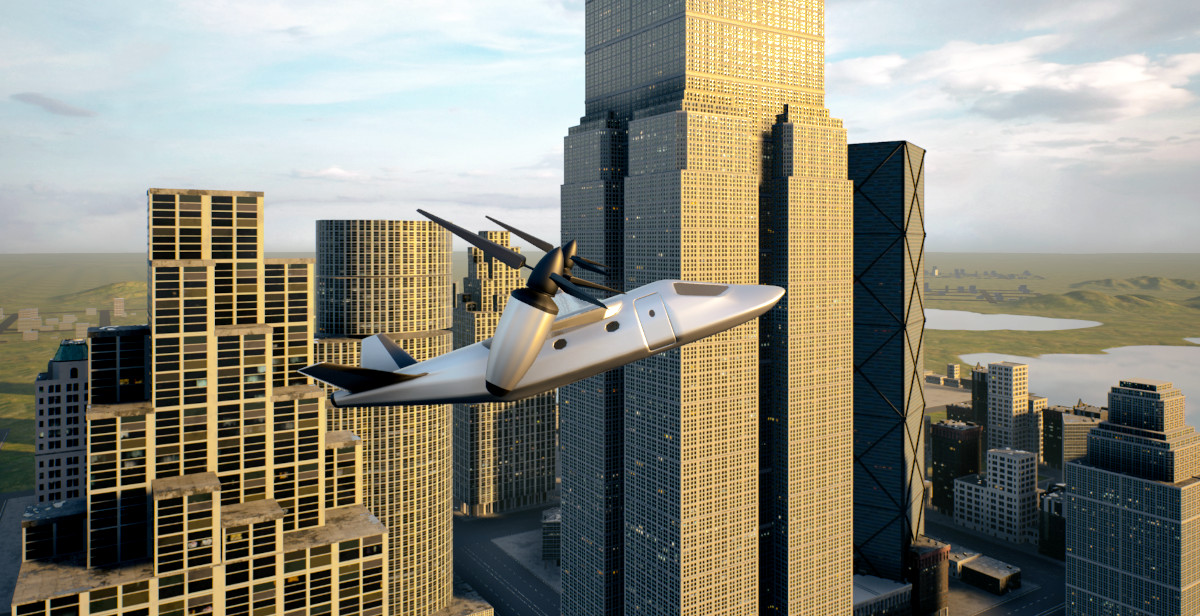
\includegraphics[width=\textwidth]{figures/vtol_airsim_cityblocks_crop3}
    \caption[Tiltrotor vehicle in CityBlocks environment]{
        \textit{VTOL-AirSim}: our tool for simulating eVTOL aircraft in realistic environments.}%
    \label{fig:vtol_airsim_cityblocks}
\end{figure}

Advancements in computing power, electronics, digital sensors, and software have enabled great progress towards increasingly automated flight of these aircraft, which is further made possible by their fully electric propulsion. With autonomous flight capabilities, eVTOLs will have greater safety, efficiency, and ease of operation. Key to the research and development of autonomous vehicles is the ability to simulate their control and navigation software; however, because they have only recently become a possibility, the field of eVTOL research is less mature, and simulators with support for eVTOLs are scarce.

Many modern unmanned aerial vehicles (UAVs) that can fly autonomously rely on camera sensors. This is because visual data contains a large amount of information about the environment that can be used to detect and avoid obstacles, navigate through cluttered spaces, and identify and track targets. It is therefore important to simulate vision-based navigation for eVTOLs. Simulating visual data from a camera sensor, however, requires high-fidelity graphics to accurately test the performance of the vision-based navigation software. There are few publicly available simulators which utilize high-quality graphics engines, and this further complicates finding a viable simulator for eVTOLs.


% There is also great variation in eVTOL designs, and so including the category of eVTOLs into a simulator would require sophisticated customization capabilities In addition, they often have moving parts that are normally stationary on aircraft, such as tilting rotors

This thesis explains our contribution of creating a capable, high-graphics simulation of winged eVTOL aircraft that others can use. In addition, we show a system that we developed for others to easily create their own unique simulations of eVTOLs. The simulation we developed is an extension of Microsoft AirSim, a popular open-source tool used by many researchers for simulating multirotor aircraft.

% \expandafter\show\the\font

\section{Review of Available Simulation Tools}
To the best of our knowledge, there are currently no publicly available simulators for research that provide the ability to simulate eVTOL aircraft with high-quality graphics. Therefore, it was necessary for us to choose from the simulation tools that are available and design a way to modify, extend, or otherwise work around these tools to produce something that they currently do not offer.

There are two well-known products in the world of flight simulation that are renowned for their high-fidelity graphics, massive amount of features, and accurate modeling of the physics of flight: \textit{Microsoft Flight Simulator}~\cite{Microsoft2020}, and \textit{X-Plane 11} from Laminar Research~\cite{X-plane112020}. While different, these two products fit into similar categories as simulation tools. A brief comparison of the two are given in~\cite{Gimenes2008}. They offer creating customized aircraft, but with different implementations. The flight model in Flight Simulator uses a set of tables which are computed by supplied parameters. X-Plane 11 computes flight dynamics directly from the visual model, and it allows for the use of one's own flight model, in which case the aircraft becomes just a visual representation of the externally simulated dynamics. The latter is advantageous in the case of simulating an eVTOL aircraft, in which the dynamic model can greatly differ from that of standard fixed-wing, helicopter, or multirotor aircraft. However, neither software allows for winged eVTOL designs, such as animating tiltable rotors. This is undesirable --- not only for the purpose of presenting simulations to others, but also for the engineering analysis and insight that is lost when using a visualization that misrepresents core components. In addition, both simulators are closed-source, proprietary software products that are heavily geared toward simulating the piloting of aircraft rather than tools for researching autonomous navigation software for UAVs. They don't provide easy-to-use, flexible programming interfaces to accommodate typical software written by researchers. Despite this, some researchers have found them useful as UAV simulators, due to their high fidelity graphics and flight dynamics, such as the use of Microsoft Flight Simulator in~\cite{Marcu2011},~\cite{Louali2011} and the use of X-Plane in~\cite{Garcia2010},~\cite{Cho2021}. Note that these studies only simulated standard fixed-wing or helicopter aircraft.

% where they use ROS for mission state communication, but the setup required ``considerable implementation steps''

A simulator that has arguably become the standard simulator for robotics research is the free and open-source Gazebo project~\cite{Koenig2004}. It is widely used in both robotics and UAV research and thus has a large community. It is highly customizable, even to allow for simulating eVTOLs, as in~\cite{Carlson2021}. However, this comes at the cost of requiring a great deal of manual setup on the part of the researcher, as Gazebo is a rather generic robotics simulator and does not offer built-in features such as eVTOL aircraft. In addition, the graphics quality of simulations made in Gazebo are, by today's standards, of moderate or low fidelity. This makes it less useful for accurately simulating vision-based navigation and control.

Another simulator from Microsoft, \textit{AirSim}~\cite{Shah2018}, is becoming increasingly popular among multirotor UAV researchers. It is free, open-source, and is built on \textit{Unreal Engine}~\cite{Games2020}, a professional game engine from Epic Games that is known for its very high-quality graphics. It has many built-in features, such as support for the PX4 Autopilot~\cite{Meier2015} and ROS~\cite{OpenRobotics2013}, and it provides simple interfaces in Python and \CCd. It also offers a number of prebuilt environments of high-quality graphics that can be downloaded and ran on anyone's machine in a number of minutes. AirSim has been used for simulating vision-based navigation in~\cite{Ruf2018},~\cite{Bondi2018},~\cite{Meier2015}. A core problem with AirSim is that it's completely structured around three separate simulation modes: Multirotor, Car, or Computer Vision (i.e., a camera with no dynamics or vehicle). This means that eVTOL aircraft, or even fixed-wing vehicles, can not be simulated in AirSim. Moreover, while AirSim is open-source and does contain documentation on how to customize it, doing so requires installing and using Unreal Engine, which has high computer hardware requirements and a steep learning curve.

And finally, there is the \textit{ROSflight Holodeck} simulation system. This is a tool developed by the MAGICC Lab that combines two other projects, the ROSflight autopilot created by former students of the MAGICC Lab, and the Holodeck simulator, created by the BYU Perception, Control, and Cognition Lab, into a full software-in-the-loop simulation with a high-quality graphics environment. Like AirSim, Holodeck uses Unreal Engine for its graphics, and thus can be a great tool for computer vision applications. In contrast to AirSim, the project's sole developers are a few graduate students, and it currently lacks many important features, such as support for multiple vehicles.

For our solution, we chose to develop an extension to Microsoft AirSim that adds the capability of simulating eVTOL aircraft, which we gave the name of \textit{VTOL-AirSim}.

\section{Contributions}

This thesis makes contributions in the following areas:

\begin{itemize}
    \item An extension to AirSim for simulating eVTOL aircraft control and dynamics, named VTOL-AirSim. It includes high-quality graphics for realistic simulated camera images. We also created visual components for the simulation: a fully animated tiltrotor aircraft mesh, and a detailed city environment to fly it in. An introduction to AirSim and tutorials for VTOL-AirSim, which includes scripts we created for interfacing VTOL-AirSim with a trajectory generator, a geometric controller and an eVTOL control allocation module from the MAGICC Lab's VTOLsim project~\cite{Willis2021},~\cite{Willis2022}, are given in Chapter~\ref{chp:userguide}. A tutorial for interfacing the PX4 Autopilot with VTOL-AirSim is also given in that chapter.
    \item A guide on all the tools that are needed to extend VTOL-AirSim is given in Chapter~\ref{chp:extending}. We show how to build Unreal Engine from source and install it on Linux, after which we provide a short user guide.
    \item Tutorials for creating custom aircraft and custom environments for use in VTOL-AirSim are given in Chapters~\ref{chp:custom_aircraft} and~\ref{chp:custom_envs}, respectively. We provide full examples of how to obtain prebuilt content from online and then integrate the content using the Unreal Editor to create a customized VTOL-AirSim simulation.
\end{itemize}


% Advanced Air Mobility (AAM) is a new class of air transportation involving electrically powered vertical takeoff and landing (eVTOL) aircraft which promises to provide low-cost, on-demand transport of people and cargo to places not currently or easily served by existing modes of aviation. A key advantage of eVTOL aircraft is their ability to take off and land in compact or congested spaces, allowing them to perform takeoff and landing virtually anywhere, without requiring runways. They also are able to exploit the huge benefits of fixed-wing flight, which includes vastly more energy-efficient travel and faster speeds when compared to helicopters and other rotorcraft. The combination of these advantages will extend their reach to rural and suburban areas as well as complex urban environments. Developments such as cheaper, more efficient and lighter-weight battery technology has only recently made transport via electric aircraft both technically and economically feasible. Electric propulsion brings many benefits such as greatly reduced mechanical complexity, reduced manufacturing and operating costs, lower noise, zero emissions, and simplified electric controls. In addition, developments in the fields of software, sensors, and electronics has enabled great progress towards increasingly automated flight of these aircraft, which has the potential to improve their safety, easy of use, and efficiency.
%TC:envir minttcb [ignore] xall

\chapter{VTOL-AirSim User Guide}\label{chp:userguide}

This chapter will be a detailed guide involving the setup, configuration, and basic uses of Microsoft AirSim and our extension to AirSim, VTOL-AirSim. Sections~\ref{sec:description_airsim}--\ref{sec:basic_use_airsim} are written for those who have never used AirSim previously, and serves as an introduction to AirSim. Sections~\ref{sec:vtolairsim}--\ref{sec:vtol_examples} are about VTOL-AirSim and examples of how to use it.

All instructions throughout this text are written for Linux users. The instructions have been tested on Arch Linux and Ubuntu 20.04 --- the latest Long Term Support (LTS) release as of this writing --- and are written with a focus on Ubuntu users.

% The setup instructions for extending the capabilities of AirSim are covered in Chapter~\ref{chp:extending}, and setup for the Unreal Editor is covered in Section~\ref{sec:unreal_setup}.

If this is your first time using AirSim, regardless of your use case, it is recommended that you follow the setup guide described in this chapter before continuing to the advanced chapters. This will help you to be aware of the various components involved in a complete simulation environment, which will be very beneficial knowledge when debugging a problem or attempting to add functionality to the sim later.

\section{Description of AirSim}\label{sec:description_airsim}

It is important to first understand what exactly AirSim is before setting it up. AirSim should be thought of not as a single, self-contained simulator program, but rather as a collection of simulation tools which you can link together in various ways and interface with at various levels. Because of this, there are multiple ways to use AirSim, and individual AirSim-based simulations can appear to be quite different from one another depending on which components are used. Nevertheless, there are two parts to any complete AirSim simulation: an environment (the server) and one or more clients interacting with the environment. While it is technically possible to have zero clients connected to the environment server, the result would be an environment containing one or more vehicles that never perform any actions, and this is not very useful. Thus, any complete AirSim simulation has at least one connected client. What follows is a brief description of these two parts and their major components.

Note that for simplicity, the following sections are worded in terms of a single vehicle in the simulation; however, AirSim has full multi-vehicle support, so any mention of a single vehicle can be substituted with multiple vehicles. In addition, AirSim also has a car mode, but it is outside the scope of this work.

\subsection{Definitions}\label{sec:definitions}
The following terms can have different meanings depending on the context, and so we have decided on some fixed definitions for this text.

\begin{itemize}
    \item \textbf{mesh} --- The collection of vertices, edges, and faces that make up the graphical representation of an object.
    \item \textbf{model} --- The dynamic model of the vehicle; or, in other words, the equations of motion, control inputs and motor outputs that are particular to a vehicle or vehicle type.
    \item \textbf{viewport} --- The area of the screen in which rendered graphics are displayed to the user.
\end{itemize}


\subsubsection{Environment}
The environment is a 3D graphics application which has been compiled for use with AirSim. The environment contains a scene made up of various meshes, which may be static or mobile. The vehicle is an animated mesh representing the state of the aircraft which the user controls. The graphics engine rendering the environment and the vehicle is \textit{Unreal Engine}: a game engine used for producing high-end graphics video games, but which can also be a useful tool for engineering simulations. When the environment is running, Unreal Engine is responsible for the following tasks: render images for the simulated camera sensor from the environment; handle vehicle collisions with objects in the scene; animate any moving parts of the vehicle plus the movement of the vehicle itself; and display rendered images to the user's viewport. Meanwhile, invisible to the user, AirSim performs a number of other tasks, namely: simulate the physics of the vehicle and the non-camera sensors; process control inputs and simulate motor responses --- either through its own autopilot stack for multirotors, SimpleFlight, or by interfacing with an external autopilot such as PX4 --- communicate with Unreal Engine about the vehicle's state and the physics of any collisions that occur; and run a remote procedural call (RPC) server, which processes commands sent by the client.

\subsubsection{Client}
The client is a process initiated by the user which sends commands to the server (the RPC server which runs inside the environment). Any client is initiated independently from the environment. There can be multiple clients running and simultaneously passing data to and from the server. Clients can be created, shut down, or restarted any number of times while the server is running. The environment is initiated first, because it is the server, and any clients are initiated after. This is because a client won't perform any actions until a connection with the server is established, and if it tries to create a connection but can't, it will close with an error.

\subsection{Outline of AirSim Components}
We have just explained the two primary parts of an AirSim simulation: the environment and a client. With that knowledge in hand, we will now outline the major components of AirSim.

\begin{itemize}
    \item AirLib --- The core \CC code of AirSim consisting of many subcomponents, including:
    \begin{itemize}
        \item physics (dynamics, drag model, thrust and torques, collision handling)
        \item non-camera sensor models
        \item control inputs and motor responses
        \item a small, self-contained multirotor autopilot called SimpleFlight
        \item interfaces for the autopilots PX4 and Ardupilot
        \item RPC server and client
    \end{itemize}
    \item MavLinkCom --- \CC library that uses MavLink to communicate with PX4 or Ardupilot
    \item Python client --- a Python wrapper around the \CC RPC client found in AirLib
    \item Compiled environments (binaries) --- a selection of prebuilt, downloadable environments
    \item Unreal Engine plugin, plus a simple example project named Blocks
    \item Unity plugin --- a plugin for the Unity game engine, which will not be covered in this text
\end{itemize}

Each of these components may or may not be used in a given AirSim simulation, but they are all part of the stack of software that AirSim offers. It is up to the user to decide which of these components to use, interface with, or modify based on the needs of the project at hand.

\section{Basic Setup: Prebuilt Environment}\label{sec:basic_setup}

We will now begin with the most basic setup of AirSim: using a prebuilt environment. This is the least configurable way to use AirSim, but it is the fastest and easiest way to get an AirSim simulation running on your machine. Prebuilt environments allow for some configuration by way of a settings file. For some projects, the settings offered for prebuilt environments may be sufficient.

The first step is to download a prebuilt environment from the AirSim GitHub repository. The repository is located online at \url{https://github.com/microsoft/AirSim}. This is the repository containing all of the source code behind the various components outlined in the previous section. On the right of the page you will see several sections containing information about the repository. The first section is labeled \textbf{About}, and underneath it is a section labeled \textbf{Releases}. Click on the header \textbf{Releases} to go to the AirSim Releases page. Alternatively, you can go directly to the page at \url{https://github.com/microsoft/AirSim/releases}.

\subsection{Explanation of GitHub Releases}
If you are not familiar with the concept of releases, it is essentially a snapshot of the software contained in the repository at a certain moment (i.e., at a specific commit). Developers create releases at particular commits that they have deemed important enough in some way to warrant packaging the code in a deliverable format, and to give the commit a special label called a \textit{tag}. A commit can be tagged without creating a release (hence the \textbf{Tags} subsection on the Releases page), but a release is always associated with a tag. Releases are most often used to mark a version of the software. Every release on GitHub includes links to download a copy of the source code at that particular commit, but they may also include release notes or additional files for others to use. Often, the managers of a repository will include links to binary files which have been compiled from the source code at that release. This is how the AirSim developers structure their releases.

\subsection{Download an Environment}
On the AirSim Releases page, you will find links to download environments built by the AirSim team. AirSim usually creates two releases for every new version: one containing environments compiled for Windows, and another with environments compiled for Linux; the source code is the same in each. Scroll down the page until you find the most recent release for Linux. The release should be titled in the form of \texttt{vX.Y.Z --- Linux}, where X, Y, and Z are numbers making up the version of that release. For example, as of this writing, the most recent release is titled \texttt{v1.5.0 --- Linux}; it contains environments built for Linux using version 1.5.0 of the AirSim source code. Be sure that you find the release for Linux and not Windows --- although the files may have the same names, the environments listed under the Windows release are \textit{not} compatible with Linux.

Once you have found a Linux release, at the bottom of the release notes you will find all the files that are a part of the release under the expandable section labeled \textbf{Assets}. Expand this section by clicking on the label, after which you should see a number of links pertaining to each environment that has been built for Linux. (For brief descriptions of the available environments, see Appendix~\ref{apdx:list_of_envs}.) A good environment to start with is the AirSimNH environment (\textit{NH} meaning \textit{Neighborhood}). Download the ZIP file for this environment and unzip it to a directory of your choice.

Finishing this step will give you the first part of AirSim: the environment. You still need to be able to start a client before you can do anything with AirSim. To start a client, we will use AirSim's Python interface with one of the example Python scripts that AirSim provides.

\subsection{Create a Python Virtual Environment for AirSim}\label{sec:virtual_env}
If you haven't used a Python virtual environment before, it is very easy to create and use one. What it does is create an isolated space (a directory) where non-built-in Python packages will be installed to and searched for when importing or executing code from those packages. All you have to do is create the virtual environment and \textit{activate} it each time you want to use it; you then \textit{deactivate} it when you don't.

It is strongly recommended that you create an entirely fresh Python virtual environment specifically for AirSim. As of this writing, the \ci{airsim} Python package has a dependency on a deprecated and very old package named \ci{msgpack-rpc-python}, which itself has other outdated dependencies that can create problems if you integrate it with your other Python virtual environments, or your user-wide or system-wide Python environments.

% \subsubsection{Make the Virtual Environment}
You can place the virtual environment wherever you like. It is common to create a folder dedicated to storing virtual environments, often in the user's home directory. The following instructions will create a directory named \ci{.virtualenvs} in the home directory; feel free to replace the path with whichever path and directory name you choose.

First, create a directory to store virtual environments. If you already have a directory that fulfills this purpose, skip this step.
\begin{minttcb}{bash}
    mkdir ~/.virtualenvs
    cd ~/.virtualenvs
\end{minttcb}
\noindent Next, create a virtual environment. We will name it \ci{airsim}.
\begin{minttcb}{bash}
    python3 -m venv airsim
\end{minttcb}
This will create a folder at the current working directory named \ci{airsim} containing a brand new virtual environment. Note that a virtual environment can only contain a single version of Python, and the above command will create a virtual environment according to whichever Python version the \ci{python3} command points to on your system. If you need to some other Python version, replace the number 3 with the specific version you need. For example, if you need to use Python 3.9 but \ci{python3} points to Python 3.8 (verify with the command \ci{python3 --version}), replace \ci{python3} in the above command with \ci{python3.9}. \textit{Warning: be sure you are using Python 3. Do not attempt to use Python 2 with AirSim}.

% \subsubsection{Activate the Virtual Environment}
To activate the new virtual environment, you need to source its \ci{activate} script, which can be done with the following command.
\begin{minttcb}{bash}
    source ~/.virtualenvs/airsim/bin/activate
\end{minttcb}
This will do a number of things to configure your shell's environment to use the \ci{airsim} directory for importing and installing new Python packages. You have now \textit{activated} your virtual environment for AirSim. Whenever you need to use your AirSim virtual environment in the future, you must either run the above command directly, or, to make it easier to remember, you can create an alias for that command and then use the alias. To stop using the virtual environment, run the command \ci{deactivate} in the terminal.

If you would like a setup that is a bit more convenient and robust for activating and deactivating virtual environments, see Appendix~\ref{apdx:adv_setup_python_venv}.

\subsubsection{Install the AirSim Python Package}
The AirSim Python package can be installed through \ci{pip}. Activate your virtual environment, ensure that \ci{pip} is up-to-date, then install the \ci{airsim} package.
\begin{minttcb}{bash}
    source ~/.virtualenvs/airsim/bin/activate
    pip install --upgrade pip
    pip install airsim
\end{minttcb}

\subsubsection{Get the Python Client Example Scripts}
The easiest way to get all the example scripts for using the Python client from AirSim is by cloning the AirSim GitHub repository. Assuming you have added an SSH key for your machine to your GitHub account (see Appendix~\ref{apdx:github_config}), you can run the following command in a terminal to clone the repository using SSH.
\begin{minttcb}{bash}
    git clone git@github.com:microsoft/AirSim
\end{minttcb}

\section{Basic Use}\label{sec:basic_use_airsim}

This section explains the most basic method of using AirSim.

\subsection{Run the Neighborhood Environment}
Open a terminal and navigate to where you placed the \ci{AirSimNH} folder that was extracted from the \ci{AirSimNH.zip} archive, then go to \ci{AirSimNH/LinuxNoEditor}. This \ci{LinuxNoEditor} folder is created by Unreal Engine; it follows a naming convention which indicates that it is a packaged, standalone application built for Linux that doesn't require the Unreal Editor to run.

\begin{figure}[ht]
    \centering
    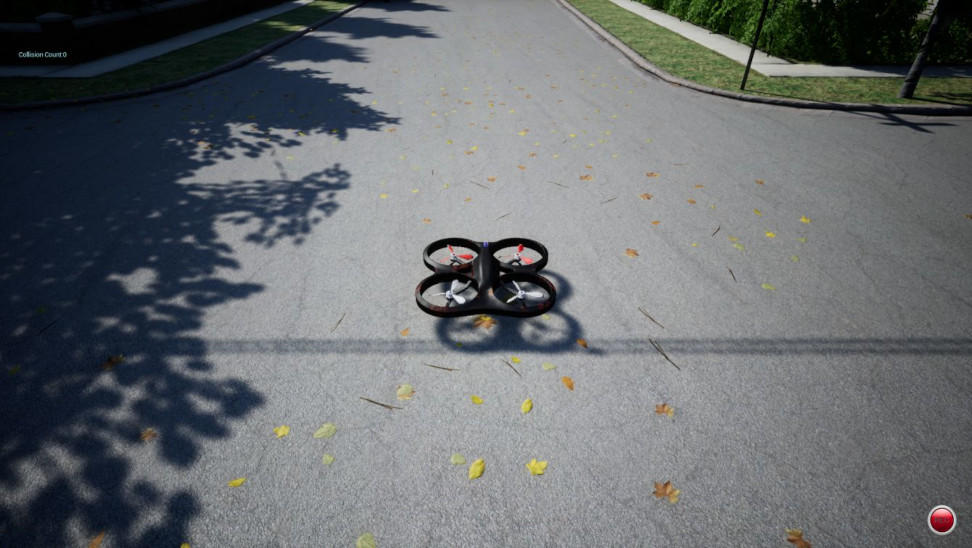
\includegraphics[height=250pt]{figures/airsimnh}
    \caption[AirSim Neighborhood Environment]{
        AirSim running in the Neighborhood environment.}%
    \label{fig:airsimnh}
\end{figure}

To start the environment, run the script \ci{AirSimNH.sh} found inside this directory. The script simply sets the application (i.e., the compiled binary) file named \ci{AirSimNH} located under \ci{AirSimNH/Binaries/Linux} to be executable, then executes it. This will start the application, and you will see a new blank window open. A dialog box will appear asking if you would like to use the car simulation. Click \textbf{No} to proceed. The window will then begin rendering the Neighborhood environment with a lone quadrotor (Fig.~\ref{fig:airsimnh}). You are now running the AirSim server. However, because there are no clients running, the quadrotor will remain stationary until a client connects and sends commands to it.

\subsection{Start the Client}
It's time to start an AirSim client. We will use one of the example scripts for using the Python client contained in the AirSim repository. Create a new terminal session and activate your AirSim virtual environment. Navigate to the directory where you cloned the AirSim repository and find the Python script \ci{AirSim/PythonClient/multirotor/takeoff.py}, then run the script. The commands for these steps are as follows:
\begin{minttcb}{bash}
    source ~/.virtualenvs/airsim/bin/activate
    cd <path to AirSim repository>/PythonClient/multirotor
    python takeoff.py
\end{minttcb}
In the AirSim window, you should see the multirotor take off, reach a certain height, then descend and land back on the pavement. Congratulations, you have just executed a complete AirSim simulation. In the next sections, we will shift our focus to VTOL-AirSim.

\section{VTOL-AirSim}\label{sec:vtolairsim}
Our additions to AirSim for simulating eVTOL aircraft is called \textit{VTOL-AirSim}. The previous sections in this chapter apply equally well to VTOL-AirSim, as it is simply AirSim with extended capabilities. From a user standpoint, the biggest difference is the addition of a new \textit{simulation mode}. AirSim's three simulation modes are: \ci{Multirotor}, \ci{Car}, and \ci{ComputerVision}. In each mode, a multirotor, or a car, or a controllable camera will spawn, respectively, and each type has its own set of control schemes. The simulation mode is specified in the settings file (Section~\ref{sec:settings_file}); or, if it isn't specified there, AirSim displays the dialog box when you start an environment asking if you would like to use the car simulation, after which it will start the \ci{Car} or the \ci{Multirotor} mode according to the user's selection. In VTOL-AirSim, we added a fourth simulation mode: \ci{Vtol}. In this mode, a tiltrotor vehicle will spawn, and it has its own set of control schemes, which we cover in the examples given in Section~\ref{sec:vtol_examples}.

\subsection{The Tiltrotor Model}\label{sec:tiltrotor_model}
It is important to know that the dynamic model for the tiltrotor vehicle is the E-flite Convergence aircraft (Fig.~\ref{fig:convergence}). This is because another project by the MAGICC Lab, named VTOLsim, had previously created a dynamics simulation utilizing a model of the Convergence aircraft. Given that we already had the various physical and aerodynamic parameters of the model, we had the actual hardware, and the Convergence was one of the airframes supported by the PX4 Autopilot, we chose to use it for the first iteration of an eVTOL vehicle in AirSim.

\begin{figure}[ht]
    \centering
    \begin{subfigure}[b]{0.42\textwidth}
        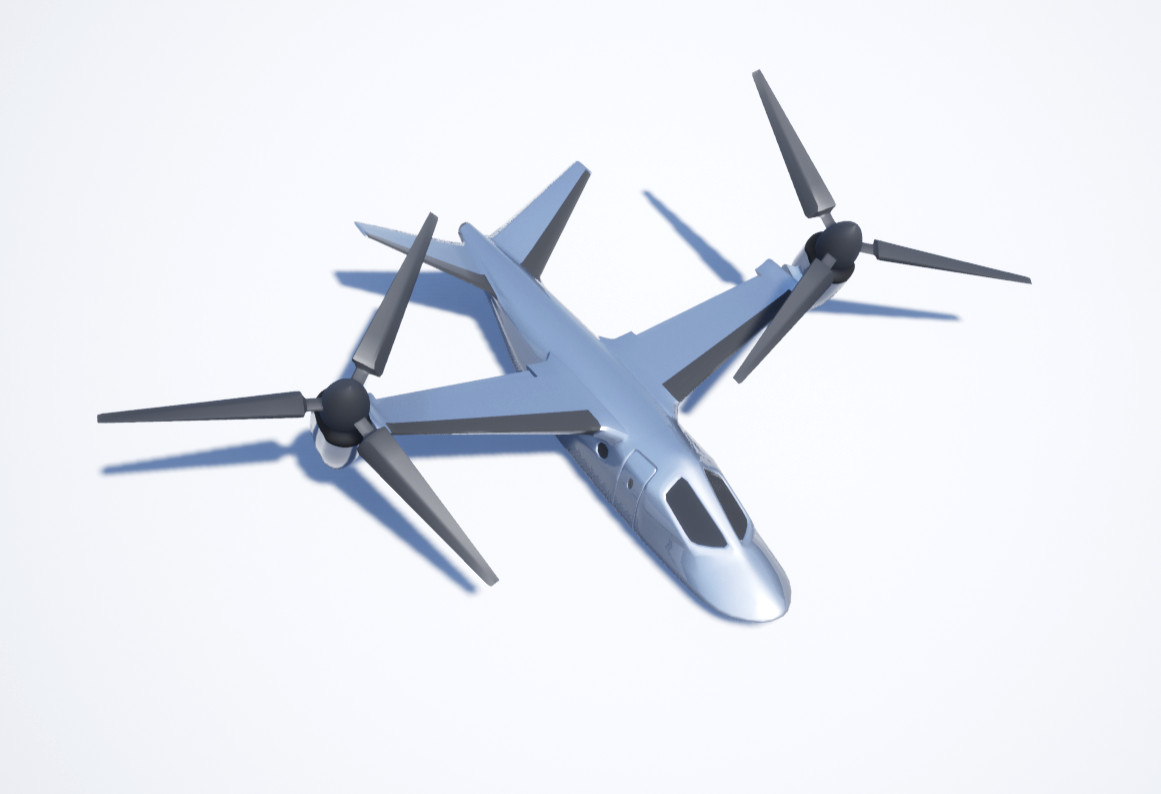
\includegraphics[width=\textwidth]{figures/tiltrotor_solo3}
        \caption[Tiltrotor vehicle used in VTOL-AirSim]{
            The tiltrotor vehicle in VTOL-AirSim.}%
        \label{fig:tiltrotor_solo}
    \end{subfigure}
    \qquad
    \begin{subfigure}[b]{0.42\textwidth}
        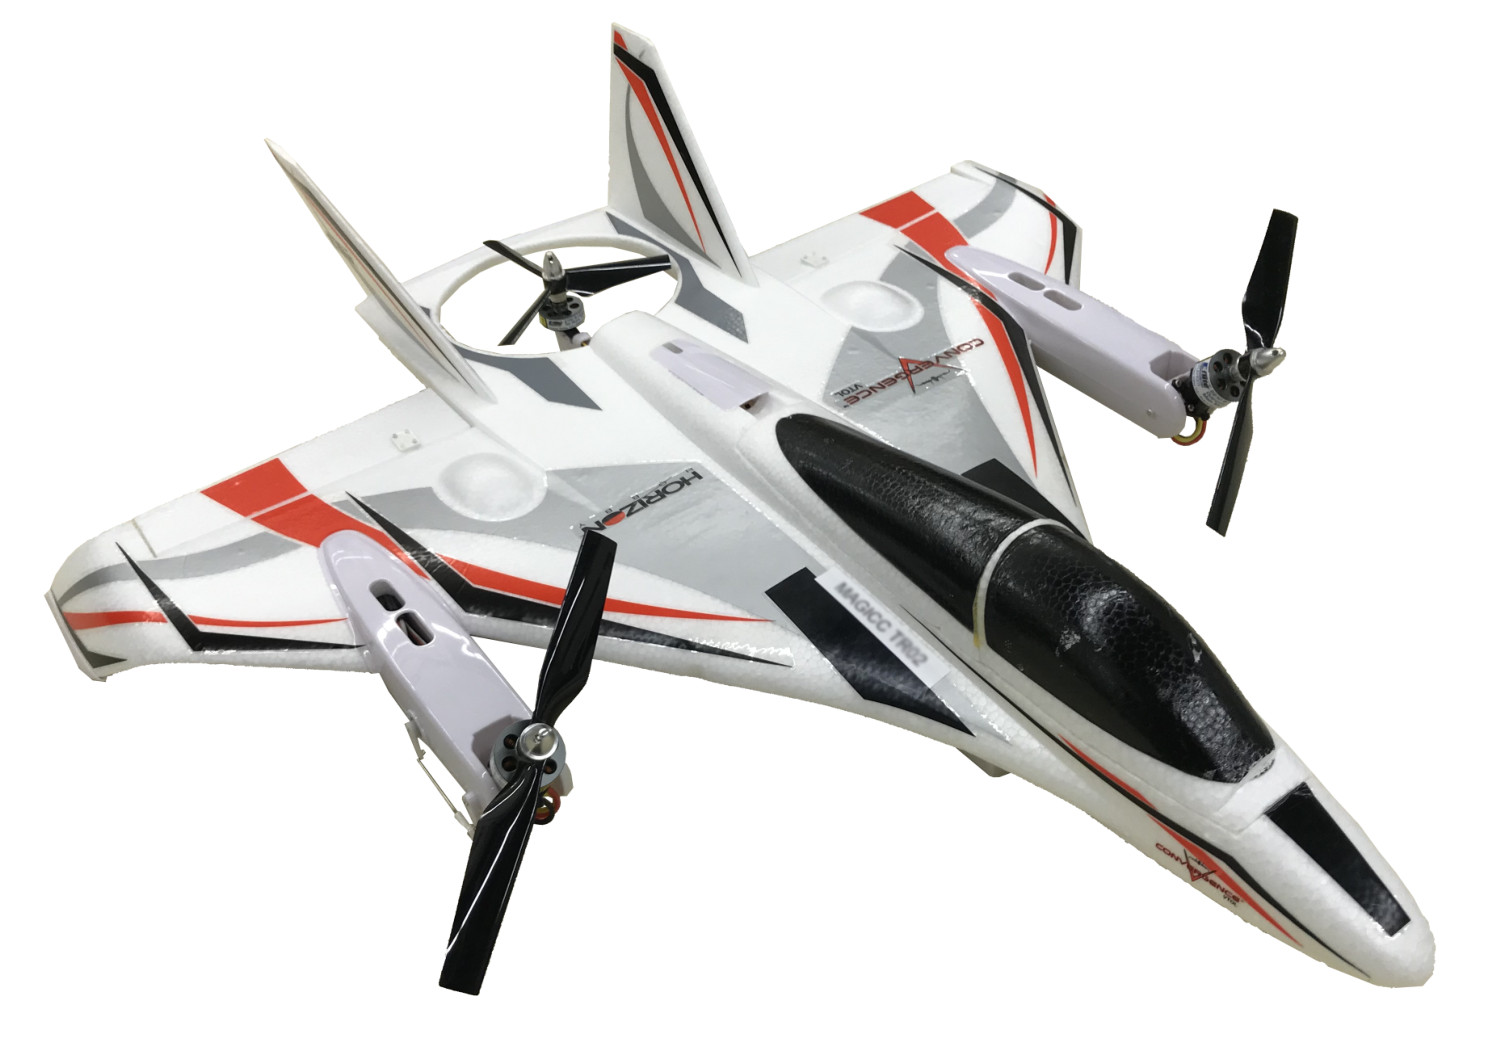
\includegraphics[width=\textwidth]{figures/convergence}
        \caption[E-flite Convergence aircraft]{
            The E-flite Convergence aircraft that serves as the dynamic model.}%
        \label{fig:convergence}
    \end{subfigure}
    \caption[Tiltrotor vehicle in VTOL-AirSim compared with E-flite Convergence]{
        Comparison of the tiltrotor mesh in VTOL-AirSim and the E-flite Convergence.}%
    \label{fig:tiltrotor_convergence}
\end{figure}

Note that the Convergence actually has three rotors --- it is a \textit{tri-tiltrotor} design --- but the tiltrotor in VTOL-AirSim only has two. We were not able to find a suitable mesh for a tri-tiltrotor aircraft when we created the tiltrotor vehicle. In addition, the Convergence is a small UAV that requires a rear rotor for stability, while a passenger-size tiltrotor would typically not have a rear rotor, so we decided that this was acceptable. However, internal to VTOL-AirSim, the tiltrotor does in fact have a rear rotor; it is simply not a part of the visual representation.


\subsection{Environments Available in VTOL-AirSim}
One component of AirSim that is not shared by VTOL-AirSim is the availability of AirSim's prebuilt environments. Because we do not have access to the Unreal Engine assets that the AirSim developers used to create their environments (other than the Blocks environment), VTOL-AirSim can't be compiled into, say, the Neighborhood environment. There are, however, two environments which we have compiled for VTOL-AirSim: Blocks, and CityBlocks. More information on the CityBlocks environment is in Section~\ref{sec:download_cityblocks}, and this is the environment we use in the VTOL-AirSim examples.

\section{The Settings File}\label{sec:settings_file}

There are many settings available for configuring the AirSim environment. All settings for AirSim are placed in a \ci{settings.json} file at the path \ci{~/Documents/settings.json}. For the official documentation on most of the available settings, go to \url{https://microsoft.github.io/AirSim/settings}. This section will outline the most important configuration options for VTOL-AirSim pertaining to eVTOL aircraft.

\subsection{Settings Are Read at Runtime}
At startup, AirSim checks for a JSON file at \ci{~/Documents/settings.json}, then, if it exists, it reads the file's contents and attempts to apply all the settings that are recognized. The settings file is read at the time of initialization; in other words, it is performed at runtime. This means that if a value for any setting is invalid, the application will generally crash during startup. In addition, the file must strictly follow official JSON syntax; if there are any syntax errors, the JSON parsing library that AirSim uses will throw an exception of type \ci[cpp]{std::invalid_argument}, causing the application to crash without printing any helpful information as to why it crashed. Be aware of this when you edit the settings file, and know that this is a common cause of startup crashes.

A key-value entry (i.e., a setting and a chosen value for that setting, which are written in the format \ci[text]{"key": "value"}) is valid if the AirSim environment was compiled with support for it. For example, the entry \ci[text]{"SimMode": "Vtol"} is valid only if using an environment that was compiled with VTOL-AirSim. If you specify that same entry and then run one of AirSim's prebuilt environments, the application will crash at startup because AirSim does not include \ci[text]{"Vtol"} as a possible simulation mode in its source code.

\subsection{Settings for VTOL-AirSim}
With the addition of the new \verb|Vtol| simulation mode, several new configuration options were added. The affected settings are outlined in the following list.

\begin{itemize}
    \item \ci{SimMode}
    \begin{itemize}
        \item Added new possible value: \ci{Vtol} (case insensitive)
        \item Explanation: Set the value to \ci{Vtol} to fly an eVTOL aircraft (currently tiltrotor only).
    \end{itemize}
    \item \ci{Vehicles}\ldots\ci{VehicleType}
    \begin{itemize}
        \item Added two new possible values: \ci{VtolSimple}, \ci{PX4Vtol} (case insensitive)
        \item Explanation: The default is \ci{VtolSimple}, which runs dummy firmware that simply passes through any PWM commands sent to it. Set this to \ci{PX4Vtol} to run VTOL-AirSim with PX4, as in the example in Section~\ref{sec:vtol_px4}.
    \end{itemize}
\end{itemize}

\section{How to Fly eVTOL Aircraft --- Examples}\label{sec:vtol_examples}
In this section we walk you through several complete examples of flying eVTOL aircraft in VTOL-AirSim. In the first example (Section~\ref{sec:vtol_geometric_control}), we cover a full demonstration that includes trajectory generation and following by sending PWM commands to AirSim. In the second example (Section~\ref{sec:vtol_teleport}), rather than sending control inputs to AirSim, we show how to override the vehicle's state in AirSim --- also referred to as \textit{teleporting} the vehicle --- for the case of utilizing an external dynamics simulation. In the third example (Section~\ref{sec:vtol_px4}), we show how to integrate the PX4 Autopilot in which we create and send a mission for the PX4 flight controller to execute and fly the aircraft.

As with the other simulation modes in AirSim, VTOL-AirSim comes with one mesh for the \verb|Vtol| vehicle in the form of a simple tiltrotor. Therefore, this is the aircraft that we use in each of the examples. We will also use the CityBlocks environment in these examples, which is one of two environments that we provide (the other being the Blocks world). If you are interested in changing what is available in VTOL-AirSim see Chapter~\ref{chp:extending} for information on how to get started.

\subsection{Required Settings}
For the first two examples in this section, \textit{Geometric Controller With PWM Commands} (Section~\ref{sec:vtol_geometric_control}) and \textit{Teleporting} (Section~\ref{sec:vtol_teleport}), you should have the following settings in your \ci{settings.json} file. As always, it should located at \ci{~/Documents/AirSim}.
\begin{minttcb}[title={Required Settings for eVTOL Examples}]{json}
{
  "SettingsVersion": 1.2,
  "SimMode": "Vtol",
  "ClockSpeed": 1.0,
  "LogMessagesVisible": false,
  "Vehicles": {
    "uav0": {
      "VehicleType": "VtolSimple"
    }
  }
}
\end{minttcb}

You can lower the \ci{ClockSpeed} setting if it appears that your machine is struggling to run the simulation. Also, the setting \ci{"LogMessagesVisible": false} is optional; however, when recording video or screenshots for presentations, it's usually best to disable the log messages that are displayed in the window.

\subsection{Download the CityBlocks Environment}\label{sec:download_cityblocks}
The CityBlocks environment is an environment that we created for use with VTOL-AirSim that is filled with static buildings, skyscrapers, streets, fields, and water. It was purchased and downloaded from the Unreal Engine Marketplace and afterwards modified to mimic the Blocks environment file structure; hence, we gave it the name \textit{CityBlocks}.

The compiled CityBlocks environment is available on the MAGICC Lab's Box storage at \url{https://byu.box.com/v/magicc-airsim-cityblocks}. Download the ZIP file and extract the archive to somewhere on your machine. You can then run the CityBlocks application by executing the script \ci{LinuxNoEditor/CityBlocks.sh}, just as you would for the official environments provided by AirSim. In the following examples, the instruction ``run the CityBlocks environment'' means to execute this script.

\subsection{Setup for the Python Client for VTOL-AirSim}
To get the VTOL-AirSim-modified version of the AirSim Python Client, you will also need to have the BYU-MAGICC AirSim fork cloned onto your computer. In Section~\ref{sec:virtual_env}, you created a Python virtual environment specifically for AirSim. You may use the same virtual environment or you can create a new virtual environment for VTOL-AirSim. The instructions that we provide for these examples will simply use the same virtual environment named \ci{airsim.}

Inside the AirSim repository lies the directory \ci{PythonClient}. The files contained in this repository are actually what make up the \ci{airsim} Python package. We have made some additions to the package in order to command eVTOL aircraft. Run the following commands to install the modified package:
\begin{minttcb}[title={Install the \texttt{airsim} Python Package from the BYU-MAGICC Fork}]{bash}
git clone git@github.com:byu-magicc/AirSim
cd AirSim/PythonClient
source ~/.virtualenvs/airsim/bin/activate
pip install -e .
\end{minttcb}

The syntax to install a local Python package is \ci{pip install -e <path>}. The \ci{-e} flag means to install it in \textit{editable} mode. This creates a file in your virtual environment that points to the \ci{<path>} that you specify, i.e. \ci{<path to AirSim fork>/PythonClient}. Now when importing the \ci{airsim} package in Python, it will actually use the files contained in the \ci{PythonClient/airsim} folder. If you modify these files, those modifications will be read the next time you import the package.

\subsection{eVTOL Example --- Geometric Controller With PWM Commands}\label{sec:vtol_geometric_control}
In this and the next example, we will use the MAGICC Lab's VTOLsim project. This project is a repository on the MAGICC GitLab server under \url{urbanmobility/vtolsim/vtolsim}. You need to clone the repository to somewhere on your machine as well as pull down its submodules. In addition, this example was tested at the commit \ci{fc8da33}, which has been given the tag \ci{airsim_gm_ctl_ex}. We can only guarantee that the instructions given in this example work when using that particular commit. Nevertheless, you may use a newer commit if you choose to do so. You can clone, pull down the submodule \ci{trajectorygenerator}, and check out the tag \ci{airsim_gm_ctl_ex} with the following commands:
\begin{minttcb}[title={Commands to Get the VTOLsim Repository}]{bash}
git clone git@magiccvs.byu.edu:urbanmobility/vtolsim/vtolsim.git
cd vtolsim
git checkout airsim_gm_ctl_ex
git submodule update --init --recursive
\end{minttcb}

We will use the script \ci{geometric_control_airsim_sim.py}. It is a driver script which creates a VTOL-AirSim Python client for the tiltrotor vehicle (\ci{airsim.VtolClient}), generates a static spline trajectory with states parameterized by time, runs a high-level geometric controller for following the trajectory, then uses a control allocation module for producing desired rotor tilts and thrust. The tilt and thrust commands are converted to PWM commands for the individual motors which are then sent to the tiltrotor vehicle in VTOL-AirSim through the command \ci{client.moveByMotorPWMsAsync}.

In a terminal, start running the CityBlocks environment. In another terminal session, navigate to the directory \ci{vtolsim/geometric_control}. Activate your virtual environment for VTOL-AirSim, then run:
\begin{minttcb}[title={Python Script for Geometric Controller With PWM Commands}]{bash}
python3 geometric_control_airsim_sim.py
\end{minttcb}

You should see the tiltrotor take off and follow a trajectory from one rooftop to another, as seen in Fig.~\ref{fig:vtol_example_geometric}.
\begin{figure}[t]
    \centering
    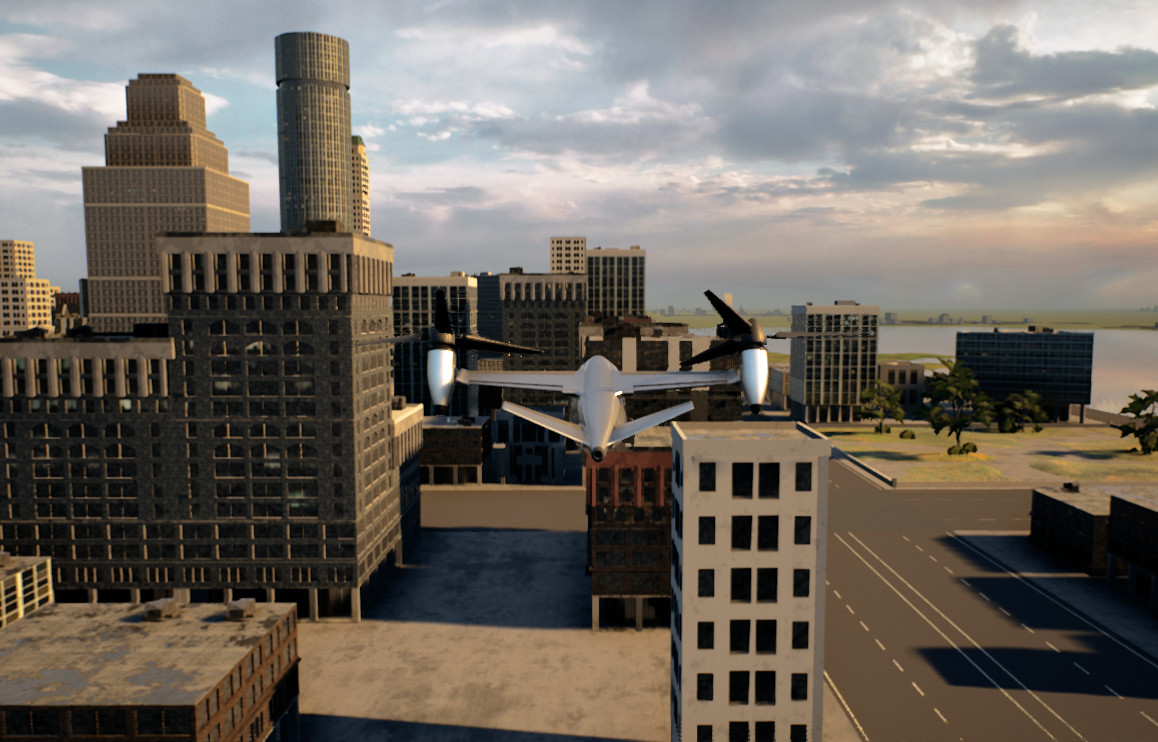
\includegraphics[height=250pt]{figures/vtol_example_geometric}
    \caption[Tiltrotor flying with geometric controller and PWM commands]{
        The tiltrotor vehicle flying in VTOL-AirSim with a geometric controller and control allocation module via PWM commands.}%
    \label{fig:vtol_example_geometric}
\end{figure}

\subsection{eVTOL Example --- Teleporting}\label{sec:vtol_teleport}
Inside the same \ci{geometric_control} directory of VTOLsim (see the previous section) is another script which does many of the same things as in the previous example, but instead of sending PWM commands to the motors, it directly sets the state of the aircraft. The script is named \ci{geometric_control_airsim_teleport.py}. It uses the same geometric controller and control allocation module, though it uses VTOLsim's dynamics simulation rather than VTOL-AirSim's. At each iteration of the main loop, VTOLsim computes the new state of the aircraft and sets the state of the aircraft in VTOL-AirSim through VTOL-AirSim's client command \ci{simSetVtolPose}. This method of using a graphics tool like AirSim for visualization of an external dynamics simulation is often referred to as \textit{teleporting}.

At the time of this writing, there are a few limitations to the teleport method. The first is that the tilt of the rotors cannot be animated. Although \ci{simSetVtolPose} has the parameter \ci{tilt_angles}, the implementation of setting the tilt angles of the rotors in this way is broken, and it produces bad results. We were not able to resolve the issue due to time constraints. For now, you should pass in values of \ci{np.nan} for the tilt angles (meaning the values won't be used), as is done in this script. The rotors will remain tilted at their \textit{nominal angle} --- set as 32.5\degree~for this aircraft --- throughout the flight. There is another parameter to the function, \ci{spin_props}, which if set to \ci{True} (the default value), should animate the spinning of the propellers, though with some minor visual artifacts.

The second limitation is that it requires using an environment compiled with a special zero gravity feature. With gravity, the aircraft can be successfully teleported to a pose in the world, but it begins falling between client calls of \ci{simSetVtolPose}. Without gravity, it stays at the commanded pose indefinitely. A version of the CityBlocks environment has been compiled specifically for this purpose, which we named \ci{CityBlocks_nogravity}. You need to download and use the latest version of the \ci{CityBlocks_nogravity} environment to run this teleport example.

in a terminal, start the \ci{CityBlocks_nogravity} environment. In another terminal session, navigate to the directory \ci{vtolsim/geometric_control}. Activate your virtual environment for VTOL-AirSim, then run:
\begin{minttcb}[title={Python Script for Teleporting}]{bash}
python3 geometric_control_airsim_teleport.py
\end{minttcb}

You should see the tiltrotor take off and travel from one rooftop to another, though without animation of the rotor tilts.

\subsection{eVTOL Example --- PX4 Integration}\label{sec:vtol_px4}
In this example, we will use the PX4 Autopilot to fly the tiltrotor. There are three items you need to run the example: the software \textit{QGroundControl}, the BYU-MAGICC fork of the PX4-Autopilot GitHub repository, and the right settings in your \ci{settings.json}.

Install QGroundControl by going to \url{https://docs.qgroundcontrol.com/master/en/getting_started/download_and_install.html}, then follow the instructions for Linux. Place the App Image file wherever you like; for example, in \ci{~/.local/bin}. Launch QGroundControl, then select your preferred units (metric is recommended).

Next, clone the \ci{byu-magicc/PX4-Autopilot} repository to somewhere on your machine, then switch to the \ci{v1.10.1-convergence} branch. We created this branch by making some additions to PX4 v1.10.1 in which we added the mixer for the E-flite Convergence airframe to the software-in-the-loop (SITL) configurations. The normal command you would run is \ci{make px4_sitl_default none_tiltrotor} to launch the PX4 firmware in SITL mode using the default tiltrotor mixer. We created the configuration \ci{none_convergence}, and this is the one you should use instead of \ci{none_tiltrotor}.

There are a number of extra settings that are needed for VTOL-AirSim to communicate with the PX4. The following settings should be in your \ci{settings.json} file:
\begin{minttcb}[title={Settings for VTOL-AirSim With PX4}]{json}
{
  "SettingsVersion": 1.2,
  "SimMode": "Vtol",
  "ClockSpeed": 1.00,
  "ViewMode": "SpringArmChase",
  "CameraDirector": {
      "FollowDistance": -20.0
  },
  "OriginGeopoint": {
    "Latitude": 40.246255,
    "Longitude": -111.647835,
    "Altitude": 1418
  },
  "Vehicles": {
    "uav0": {
      "VehicleType": "PX4Vtol",
      "Model": "TriTiltrotor",
      "UseSerial": false,
      "UseTcp": true,
      "TcpPort": 4560,
      "ControlPort": 14580,
      "Parameters": {
        "NAV_RCL_ACT": 0,
        "NAV_DLL_ACT": 0,
        "LPE_LAT": 40.246255,
        "LPE_LON": -111.647835,
        "COM_OBL_ACT": 1
      }
    }
  }
}
\end{minttcb}

The values for \ci{Latitude}, \ci{Longitude}, \ci{Altitude}, \ci{LPE_LAT}, and \ci{LPE_LON} were set for the Brigham Young University campus in Provo, Utah, USA. You may change these values to whichever location you are interested in simulating.

The \ci{ViewMode} and \ci{CameraDirector} settings are optional; however, we recommend using the \ci{SpringArmChase} mode in this example as it produces smoother visuals. You may find it useful to set this view mode in the other examples as well. Be aware that, in general, if you use \ci{SpringArmChase}, there is a bug in AirSim where the \ci{CameraDirector} is too close because of the 0.25 scale we set for the tiltrotor mesh to reduce its size. This makes it necessary to have a large value for \ci{FollowDistance}.

With the above settings, start running the CityBlocks environment. In another terminal, run the following command from within the directory containing the PX4-Autopilot repository:
\begin{minttcb}[title={}]{bash}
make px4_sitl_default none_convergence
\end{minttcb}

\begin{figure}[h]
    \centering
    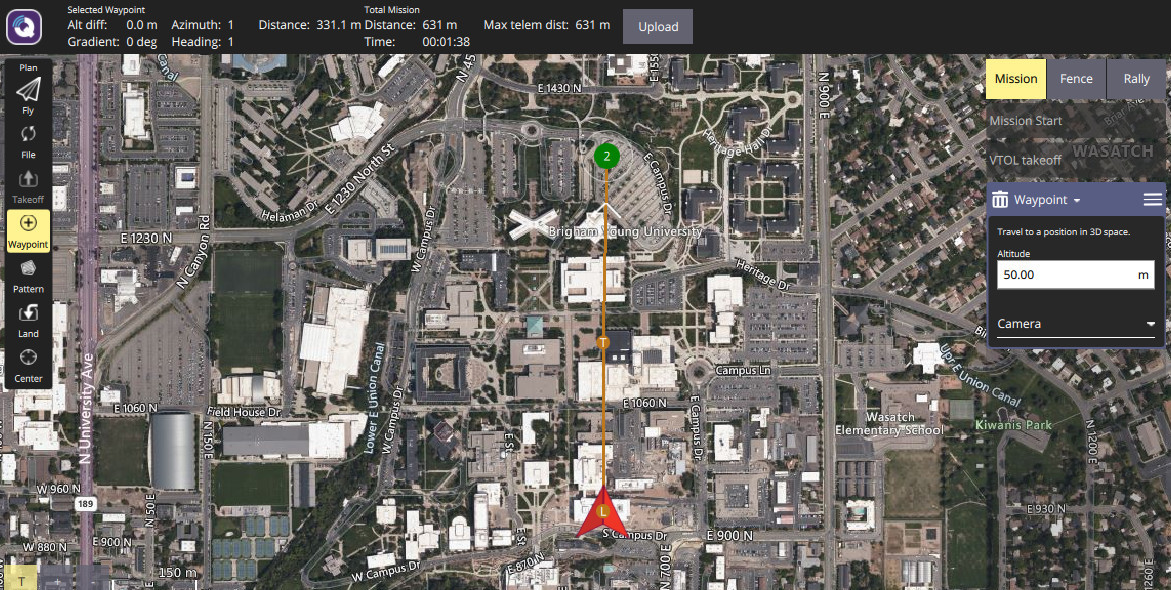
\includegraphics[width=\textwidth]{figures/qgroundcontrol_crop}
    \caption[QGroundControl showing mission plan]{
        QGroundControl screen after planning and uploading mission.}%
    \label{fig:qgroundcontrol}
\end{figure}

Next, launch QGroundControl. It should show the map centered around the detected GPS coordinate of the VTOL-AirSim vehicle (which are the values set for latitude and longitude in your settings). In the top-left of the map area, click \textbf{Plan}. Select \textbf{File} (if not already highlighted), then click \textbf{Blank}. Next, select \textbf{Takeoff}, and a green circle labeled \textbf{T} will appear (you may need to zoom out a bit to see it). You can click and drag the \textbf{T} to change the transition direction of the vehicle after takeoff, but we'll leave it there for this example. Click \textbf{Done} inside the \textbf{VTOL takeoff} box. Select \textbf{Waypoint}, then click somewhere to the north of the \textbf{T} circle. Finally, click \textbf{Upload Required} to upload the mission.  Your QGroundControl screen should look like Fig.~\ref{fig:qgroundcontrol}.

Now click \textbf{Fly}. There should be a slider button on the bottom that says \textit{Slide to confirm}. Slide the button to the right to send the mission to the tiltrotor in VTOL-AirSim. The tiltrotor should begin executing the mission (ignore any warning or error dialogs that pop up). It will first try to reach the target takeoff altitude, 50 m by default, then it will transition into fixed-wing mode in the direction that you set using the \textbf{T} circle. After that, it will head to the waypoint that you set, then after arriving, it will loiter about this waypoint --- i.e., orbit the waypoint indefinitely. It may actually hit a building while executing the mission; to avoid this, you can raise the altitude of the waypoints when planning the mission, or choose different waypoints.

\begin{figure}[h]
    \centering
    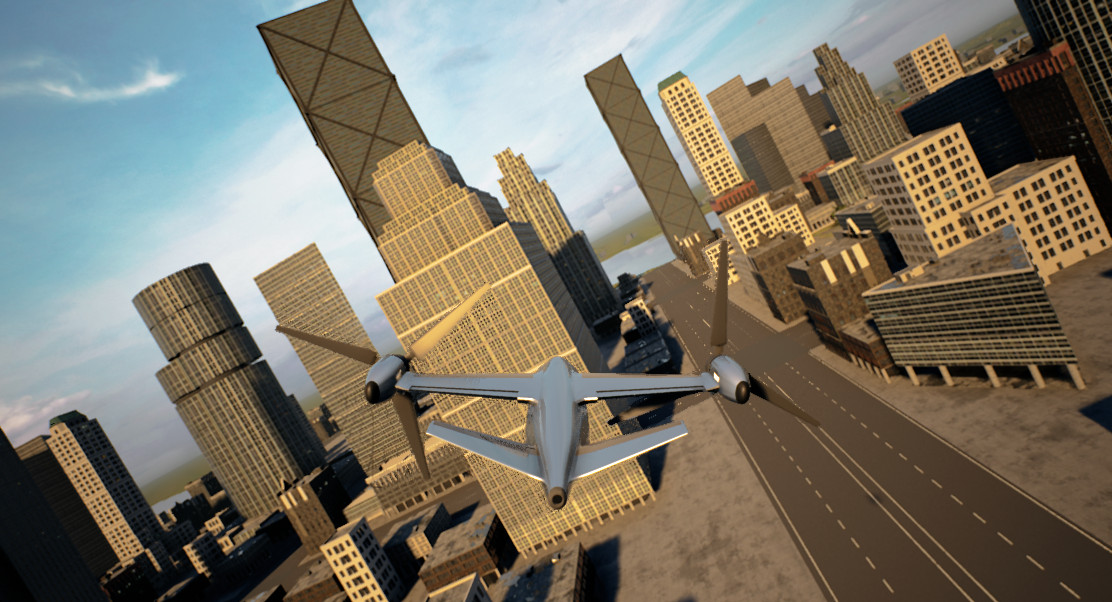
\includegraphics[width=\textwidth]{figures/vtol_example_px4}
    \caption[Tiltrotor flying with PX4 Autopilot]{
        The tiltrotor vehicle flying in VTOL-AirSim with the PX4 VTOL controller.}%
    \label{fig:vtol_example_px4}
\end{figure}
%TC:envir minttcb [ignore] xall

\chapter{Extending VTOL-AirSim: First Steps}\label{chp:extending}

This chapter is structured as a guide to developing eVTOL simulations with VTOL-AirSim and Unreal Engine 4 (UE4). The focus will be on extending the capabilities of VTOL-AirSim and understanding more of the VTOL-AirSim framework.


\section{Introduction}
Extending AirSim --- in other words, modifying or adding anything to AirSim --- involves conducting an orchestra of many diverse tools and components that all must play together in harmony to be successful. There are a number of basic components which are required in all cases, and a few components that may or may not be required depending on the needs of the project.

At some point, you will need to use \textit{Unreal Engine} --- more specifically, the \textit{Unreal Editor} --- for testing your work. In addition, you will need to integrate your work with the existing framework of VTOL-AirSim. Your project needs may also require extending the source code. Editing the source code requires a text editor: while you may use any text editor you like, we recommend Microsoft's \textit{VS Code}, for which we provide instructions for setup and use. If your project requires customizing the graphical representation of a vehicle or the environment, then you may also need to use a specialized tool for manipulating 3D computer graphics, for which we recommend the free software \textit{Blender}.

The setup process for this orchestra of tools is significantly more involved than the basic setup explained in Section~\ref{sec:basic_setup}. In this chapter, we assume that you have read Chapter~\ref{chp:userguide} (or that you understand the concepts from the chapter), and have completed the basic setup in Section~\ref{sec:basic_setup}. We begin with instructions for setting up the two core pieces for development: Unreal Engine (Section~\ref{sec:unreal_setup}) and VTOL-AirSim (Section~\ref{sec:vtolairsim_setup}).

\section{Unreal Engine Setup}\label{sec:unreal_setup}
Unreal Engine is a game engine developed by Epic Games, Inc. Its source code is written in \CC and is an open-source project on GitHub. It is known for its high-end graphics capabilities, and while it is typically used to produce video games, it has recently found use in other industries such as film, architecture, and engineering.

For our purposes, it has several advantages over a number of other game creation tools, namely that it is free for non-commercial use, has Linux support, is written in \CC and is open-source, and it has an online marketplace with a wide selection of content available to download. It also comes with a few disadvantages, including hefty system requirements, such as a moderately powerful CPU plus dedicated GPU, at least 8 GB of RAM, and at least 100 GB of available disk space on Linux. It can take well over two hours to build Unreal Engine and the Editor from source (it is required to do so on Linux) and a large amount of time to package an Unreal Editor project into a standalone application. Opening the \CC code of an Unreal Editor project with an IDE or a text editor with code analysis can be very demanding on your system due to the immense size of the code base. Furthermore, the learning curve to use the Unreal Editor is steep, and grasping the \CC API is an equally massive undertaking.

That being said, the most important reason we are using Unreal Engine is that it is the central graphics engine used by AirSim, and it was also chosen by the BYU Perception, Control and Cognition Lab for the Holodeck simulator, which we have experience with. AirSim has recently added support for the Unity game engine; however, at the time of this writing, support for it is still experimental.

\subsection{Requirements}\label{sec:unreal_requirements}
To build Unreal Engine from source, two things are required: at least 100 GB of available disk space to clone and build the engine, and your GitHub account must be a member of the \verb|EpicGames| GitHub organization. We will explain here how to meet the latter requirement.

Unreal Engine is open-source and its source code is contained in the GitHub repository \url{https://github.com/EpicGames/UnrealEngine}. However, the repository is private, and to gain access to it you must become a member of the \verb|EpicGames| GitHub organization. The instructions for becoming a member are as follows:

\begin{enumerate}
    \item Create a GitHub account if you don't already have one.
    \item Set up SSH access to GitHub (for instructions, see Appendix~\ref{apdx:github_config})
    \item Create an Epic Games account at \url{unrealengine.com}.
    \item Follow the instructions listed at \url{https://unrealengine.com/en-US/ue4-on-github} for linking your GitHub and Epic Games accounts.
    \begin{itemize}
        \item When asked, accept the End User License Agreement for \textbf{Creators}.
    \end{itemize}
    \item Join the \verb|EpicGames| GitHub organization via the email invite. You should now have access to the Unreal Engine GitHub repository.
    \item Verify by going to \url{https://github.com/EpicGames/UnrealEngine}, and you should be able to see the repository.
\end{enumerate}

\subsection{Build the Engine and Editor}
Now clone the Unreal Engine repository into a folder of your choice and build it by running the following commands. As of this writing, Unreal Engine 4.25 is the version supported by AirSim, which corresponds to the \ci{4.25} branch of the Unreal Engine repository. \textbf{Note}: Unreal Engine is very large; cloning the repository can take between 5--30 minutes, and the build process commonly takes about two hours.
\begin{minttcb}[title={Clone and Build Unreal Engine}]{bash}
    git clone -b4.25 git@github.com:EpicGames/UnrealEngine.git
    cd UnrealEngine
    ./Setup.sh
    ./GenerateProjectFiles.sh
    make
\end{minttcb}
If the build process finishes without any errors, then the engine and the Unreal Editor have successfully been built and are ready to be used. After building, the executable for the editor can be found within the repository at \ci{Engine/Binaries/Linux/UE4Editor}. To start the editor, simply execute that file in a terminal.

\section{VTOL-AirSim Setup}\label{sec:vtolairsim_setup}
The VTOL-AirSim project is a composite project that is structured, at the highest level, as an Unreal Engine \textit{Plugin}: a self-contained collection of code, asset files, and data that can be added to (or removed from) any Unreal Engine project. It is accessible as a GitHub repository at \url{https://github.com/byu-magicc/vtol-AirSim}. The VTOL-AirSim repository began as a copy of the AirSim Unreal Engine Plugin, found inside the official AirSim repository in the folder \ci{Unreal/Plugins/AirSim}, plus the AirLib code, found in the top-level folder \ci{AirLib}. From that starting point, many additions were made, along with a handful of modifications to the original code. Our work eventually resulted in the creation of a fully functional new vehicle type in AirSim for eVTOL aircraft.

Two components of the VTOL-AirSim project exist outside of the VTOL-AirSim repository: a number of large Unreal Engine asset files stored on the MAGICC Lab's Box account, and a fork of the AirSim repository found at \url{https://github.com/byu-magicc/AirSim}. To learn more about the MAGICC Lab's fork of AirSim, see \ci{MAINTENANCE.md} in the VTOL-AirSim repository.

In this text, we normally use the term \textit{VTOL-AirSim} to refer to the entire VTOL-AirSim project, as opposed to the repository itself. In the latter case, we refer to it as the \textit{VTOL-AirSim repository} if greater clarity is needed.

The full setup instructions can be found in the \ci{README.md} document of the VTOL-AirSim repository, which you can view by going to the repository's main webpage. The instructions stated there are rather detailed, so we will not repeat them in this text. Upon completing this setup, you will have the Unreal Editor running on your machine with the Blocks example project opened. The next section will detail what you need to know for working with VTOL-AirSim in the Unreal Editor.

\section{VTOL-AirSim in Unreal Editor}\label{sec:vtolairsim_unreal}

This section will serve as a concise guide on the most important concepts for using the Unreal Editor with VTOL-AirSim. The Unreal Editor is a very sophisticated software tool which is much too broad to be covered in any amount of detail in this text. Therefore, we will only cover that which is required for you to be able to do basic work with VTOL-AirSim in Unreal Editor.%
\footnote{For more information on using Unreal Editor, see the UE4 documentation at \url{https://docs.unrealengine.com}. There are also many free resources online such as web articles and YouTube videos that cover these topics.} %
In this section, we will briefly explain the key parts of the editor interface, how to run simulations in the editor, and how to package projects into standalone applications. More advanced use of the editor for customization of aircraft and environments are covered in Chapters~\ref{chp:custom_aircraft} and~\ref{chp:custom_envs}, respectively.

\subsection{Intro to Unreal Editor}
The Unreal Editor is the main graphical user interface (GUI) tool for developing video games (or engineering simulations) that use Unreal Engine. For our goals of simulating eVTOL aircraft in photorealistic environments, there are two main purposes for which the Unreal Editor is required: to \textit{modify} the graphical aspects of the simulation, and to \textit{test} modifications --- both modifications to the graphics as well as to the underlying \CC code. This means that if your project requires any customization beyond what is offered by VTOL-AirSim, then you will need to use Unreal Editor to accomplish that.

By now, you should have built and ran the Unreal Editor on your machine. When you first open the Blocks project in the editor, you will need to wait for some shaders of the Blocks environment to be compiled. Once that has finished, you will see a screen like that shown in Fig.~\ref{fig:ueditor_first_view}. Note that the interface is divided into six different \textit{panels}. In the top-left corner of each panel is a tab element which contains the name of that panel.

What follows is a quick description of each of these panels. But first, know that in UE4, a \textit{level} is the scene (or the environment, in AirSim terms) which contains every object that you see or interact with. A game is often made up of various levels; however, in our AirSim simulations, we will only have one level. When dealing with Unreal Editor, we will use the proper UE4 term of \textit{level} rather than \textit{environment}.

\begin{figure}[t]
    \centering
    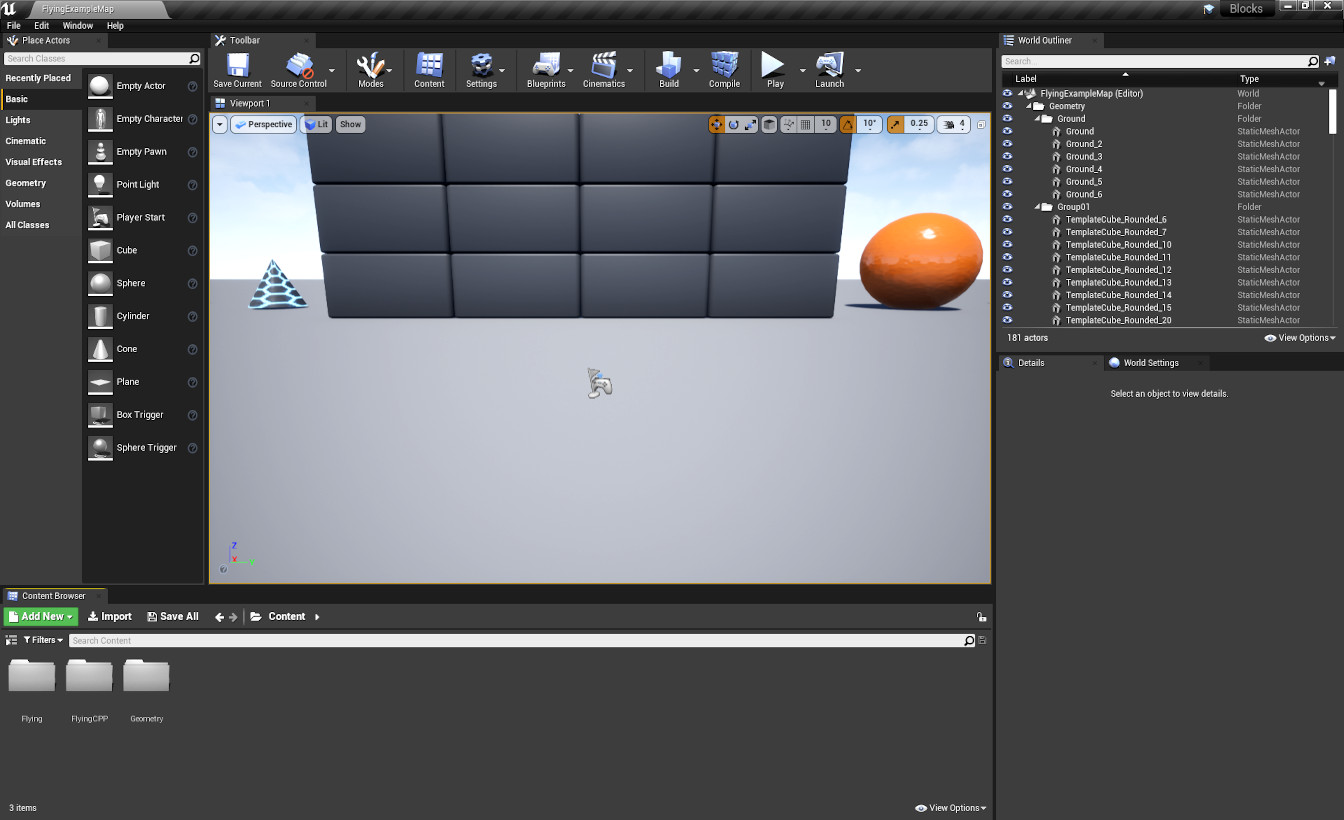
\includegraphics[width=\textwidth]{figures/ueditor_first_view}
    \caption[Unreal Editor first view]{
        The Unreal Editor with the Blocks project opened.}%
    \label{fig:ueditor_first_view}
\end{figure}

\begin{itemize}
    \item \textbf{Level Viewport} --- The center and largest panel. Here you can see and navigate around the level that the vehicle will interact with during the simulation. Because the simulation is not running, there are no vehicles visible yet. A vehicle will only spawn in the world once a simulation has started. When you press the \textbf{Play} button to begin a simulation, the \textbf{Level Viewport} will display the simulation just as it would appear in the window of a compiled environment.
    \item \textbf{Toolbar} --- Directly above the \textbf{Level Viewport}, this is where you will find the \textbf{Play} button that allows you to run a full simulation for testing (also referred to as \textit{Play In Editor} or \textit{PIE}). The other tool buttons may be ignored.
    \item \textbf{World Outliner} --- located in the upper-right of the window. This panel lists all of the \textit{Actors} that are in the scene. Actors in UE4 are any object that can be placed into a level, such as cameras, light sources, or static meshes. Currently, it only contains the Actors that are always present, but once you enter Play mode, it will additionally show dynamically spawned Actors such as one or more vehicles and the Camera Actors associated with them. Outside of Play mode, the most important Actor to be aware of is the \textbf{PlayerStart} Actor: its \textit{Location} and \textit{Rotation} (the terms in UE4 used for position and orientation, respectively) in the level are used by AirSim as the position and orientation for its internally-computed global coordinate frame. This means you can move \textbf{PlayerStart} to change where vehicles spawn in AirSim as well as what is set as the global (0, 0, 0) position and orientation.
    \item \textbf{Details} --- located in the lower-right of the window. When you click on an Actor in either the \textbf{Level Viewport} or the \textbf{World Outliner}, its configurable attributes will be found here. The key item to note in this panel is that here you can modify the \textit{Transform} of an Actor, which includes its Location, Rotation, and Scale attributes.
    \item \textbf{Place Actors} --- located at the left of the window. This panel contains a number of Actors provided by UE4 which you may place in the level.
    \item \textbf{Content Browser} --- located at the bottom of the window. Here you will find all the \textit{Assets} (or \textit{content}) that are part of the currently opened Unreal Project. The terms \textit{Assets} and \textit{content} as well as the Content Browser are covered in the next section, Section~\ref{sec:content_vtolairsim}.
\end{itemize}

\subsection{Content of VTOL-AirSim}\label{sec:content_vtolairsim}
This section will cover the UE4 content that is part of VTOL-AirSim. In UE4, the term \textit{content} refers to the objects or functionalities that make up a game (i.e., simulation) that is not \CC code. Examples of content types include Textures, Materials, Static Meshes, or Blueprints. An \textit{Asset} is a binary file that stores content. The \textbf{Content Browser} is like a special file manager that shows you all the assets that are part of the project.

By default, the editor will have open the \ci{Content} folder of the project. In our case, this is the folder \ci{Blocks/Content}. To more easily view the directory structure, click on the small icon to the left of \textbf{Filters} to reveal the \textbf{Sources panel}. You will find that the files and folders located in \ci{Blocks/Content} and in the Content Browser mostly match, with some files and folders hidden from view. The assets that we are actually interested in are not in \ci{Blocks/Content}, however, but rather in \ci{Blocks/Plugins/vtol-AirSim/Content}. To instead view these files, click on \textbf{View Options} at the bottom-right of the \textbf{Content Browser}, and check the box for \textbf{Show Plugin Content}. The \textbf{Sources panel} should now show a new folder named \ci{AirSim Content}. This folder is so named because the VTOL-AirSim Plugin actually retains its original title of \texttt{AirSim} within Unreal Engine; but it is in fact the folder \ci{Blocks/Plugins/vtol-AirSim/Content}. See Appendix~\ref{apdx:unreal_paths} for more information on path names in UE4.

There are 3 directories inside \ci{AirSim Content} that we wish to highlight:
\begin{enumerate}
    \item \ci{Blueprints} --- Here you will find the \textit{Blueprints} of several very important Actors in AirSim; in particular, the Actor for the multirotor vehicle, \ci{BP_FlyingPawn}.
    \item \ci{Models/QuadRotor1} --- This folder contains the Static Meshes, Materials, and Textures that compose the multirotor vehicle, which are specified in \ci{BP_FlyingPawn}.
    \item \ci{VTOL} --- All assets that are unique to VTOL-AirSim are contained here. Currently there is only one subdirectory, \ci{Tiltrotor}, however any custom eVTOL aircraft that may be added will go here. Inside the \ci{Tiltrotor} folder is all of the assets that make up the tiltrotor vehicle, including the equivalent \ci{BP_TiltrotorPawn} Blueprint and the Static Meshes and Materials that it is composed of, similar to the multirotor vehicle.
\end{enumerate}

Another asset, the \ci{AirSimAssets} Level, is important specifically for packaging a project, as is explained in Section~\ref{sec:packaging}.

\subsection{Play In Editor}
The most useful feature of the editor for our purposes is \textbf{Play In Editor} (\textbf{PIE}), accessed via the \textbf{Play} button. This is how you will test changes you've made to VTOL-AirSim, whether they are graphical changes made in the editor, or changes made to the source code (though changes to the code will require closing the editor and rebuilding the project before they will be active). Play In Editor allows you to preview a VTOL-AirSim simulation just as you would see in a standalone application, but displayed within the \textbf{Level Viewport}. It also has a few extra features, such as \textbf{Pause} to pause the simulation, and \textbf{Eject} to become a third-person observer where you can click on objects in the scene, such as the aircraft in the simulation, and see real-time attributes about it in the \textbf{Details} panel. For example, you could select the tiltrotor vehicle's engines to see their exact angle values while the simulation is running, and see the values change in real time. Keep in mind that you won't have the same performance using Play In Editor that you will when running a standalone application, but you should still have decent performance.

\subsection{Package a Project}\label{sec:packaging}
When you are satisfied with the changes you've made to VTOL-AirSim or your Unreal Project, you can package your project into a standalone application. This is how the compiled environments from AirSim and VTOL-AirSim are made. This allows you to get more performance out of your simulation as well as share your simulation environment with others.

There is an interesting quirk about the AirSim Plugin in Unreal Engine that is very important to know if you are going to package your project. Notice how in the \textbf{World Outliner} panel there are no tiltrotor, multirotor, or car vehicles in the scene. This is because in AirSim the vehicles that are part of the simulation are spawned at runtime; they are not permanent objects in a level. However, in Unreal Engine, only the Actors which appear in at least one level are packaged into a game. Therefore, the tiltrotor, multirotor, and car vehicles of AirSim must be present in at least one level at the time of packaging. If you specify a simulation mode in your settings file but that specific vehicle was not a part of any level, then the application will crash with an error that says \ci{Couldn't find file for package} proceeded by the path to the vehicle's Blueprint, as specified in the source code.

AirSim's solution to this is the \ci{AirSimAssets} Level, found under \ci{AirSim Content}. Double-click this level to open it, and you will see in the \textbf{World Outliner} these three vehicles, plus the Actor for \ci{ComputerVision} mode. The \textbf{Level Viewport}, however, will be completely empty and black; this is because the level contains no lighting, as it doesn't need any. It is simply a dummy level to work with Unreal Engine's packaging system.

In order to package the tiltrotor vehicle into compiled environments, we had to add the tiltrotor's Blueprint, \ci{BP_TiltrotorPawn}, to this level. If you create a custom aircraft, you will also need to add it to this level. You can click and drag the Blueprint of your custom vehicle anywhere onto the \textbf{Level Viewport} when this level is loaded (the location does not matter), and that is enough to comply with this UE4 requirement. Go back to the default Blocks level by navigating to \ci{Content/FlyingCPP/Maps} and double-clicking on \ci{FlyingExampleMap}.

Packaging a project is a simple, yet lengthy process. All you need to do is go to \textbf{File > Package Project > Linux > Linux}, choose a suitable directory to store your packaged environment, and then click \textbf{Open} and it will begin the process of packaging the project. The process can take over 30 minutes, even for the simple Blocks project on moderate computer hardware, so be prepared for that. Packaging is quicker if you choose the same directory the next time you package the project as it will only do an iterative build rather than build the complete project.

When the packaging process has completed, navigate inside the \ci{LinuxNoEditor} directory that was created, and run the \ci{.sh} file for your project just as you would with any compiled AirSim environment.

\section{Development Using VS Code}
VS Code is the text editor that we recommend for editing the VTOL-AirSim source code. Due to the massive size of the UE4 \CC libraries, it can be very demanding on your machine to edit using the code analysis features of VS Code; however, the cost is usually outweighed by the many benefits it brings for navigating and analyzing the \CC code.

The first thing you should do is install the C/\CC extension for VS Code. Next, rather than open specific \textit{files} to edit, you should open \textit{directories} for editing. The easiest way to do this is to run in a terminal \ci{code <path>}, where \ci{<path>} is the path to the directory you want to open for editing files in VS Code. For working with the VTOL-AirSim code, you can open your Unreal Engine Project that contains the VTOL-AirSim Plugin and that you will use for testing, or you can open the \ci{Plugins/vtol-AirSim} directory, or lastly you can open just the \ci{Source/AirLib} directory of VTOL-AirSim if you won't need to see any of the Unreal Engine code.

You need a special \ci{c_cpp_properties.json} file present that tells VS Code what directories to include when searching for \CC header or source files. Without this file, the C/\CC extension won't be able to do code analysis for any files that are outside the directory of the file currently being edited. There is a vast number of directories that make up the UE4 libraries, so you shouldn't create this file yourself. There is a script in the Unreal Engine repository that will do this for you named \ci{GenerateProjectFiles.sh}. The script is invoked with the syntax:
\begin{minttcb}[title={}]{bash}
GenerateProjectFiles.sh <path to Blocks>/Blocks.uproject -game -engine
\end{minttcb}
If you are using a project other than Blocks, replace \ci{Blocks} with the name of your project. This will create a number of files into your project's top-level directory for several different IDEs and text editors, but the files for VS Code are placed in a hidden directory named \ci{.vscode}. One of those files is \ci{c_cpp_properties.json}. It contains a great number of include directories to allow the C/\CC extension to do its job correctly. If you open your Unreal Project directory in VS Code, then you should be ready to start editing the code. However, since you won't need to edit any of the files outside of the VTOL-AirSim plugin, you can also copy the \ci{.vscode} directory to the \ci{Plugins/vtol-AirSim} directory, and then open just the \ci{vtol-AirSim} directory to reduce the number of files for VS Code to search through.

\section{Build}
You need to build all the VTOL-AirSim code in order to see your changes reflected in Unreal Editor. There is a guide document with build instructions located in the VTOL-AirSim GitHub repo at \url{https://github.com/byu-magicc/vtol-AirSim/blob/main/DEVELOPMENT.md}. The guide will teach you all you need to know about building the code.

Once you have completed all these setup steps, you are ready to begin developing and customizing VTOL-AirSim. In the next chapters, we show how you can create custom aircraft and environments for your own simulations.
%TC:envir minttcb [ignore] xall

\chapter{Custom Aircraft}\label{chp:custom_aircraft}

% Of the two, customizing aircraft is far more involved, and thus is the focus throughout the chapter.
It is quite possible that the vehicles, vehicle functionalities, or the environments that are provided by VTOL-AirSim are not sufficient for the needs of your project. In this case, there exists the option of customizing VTOL-AirSim beyond what it currently offers. This chapter and the next will teach you how to customize VTOL-AirSim. This chapter demonstrates how to create custom eVTOL aircraft, and the next chapter, Chapter~\ref{chp:custom_envs}, is dedicated to creating custom environments.

Because this topic can be quite broad, we have chosen to structure these two chapters on customization around guiding you through specific examples. Following our examples will allow you to see the entire process from start to finish. We begin with a discussion on a few general principles about meshes, after which we focus for the rest of the chapter on a specific example of taking a new eVTOL aircraft mesh all the way to flying it in VTOL-AirSim.

For dealing with meshes on Linux, we recommend the free 3D modeling software tool \textit{Blender}. See Appendix~\ref{apdx:blender} for more information about Blender and how to get it. You will need to install Blender in order to make some small adjustments to the example mesh before it can be properly used in Unreal Engine.

\section{Meshes}\label{sec:meshes}
As explained in Section~\ref{sec:definitions}, a \textit{mesh} is the collection of vertices, edges, and faces that make up the graphical representation of an object. Only one mesh is provided for each type of vehicle in VTOL-AirSim. For the \verb|Vtol| vehicle, we added a simple mesh of a tiltrotor aircraft (Fig.~\ref{fig:tiltrotor_mesh}). The UE4 assets for the aircraft are contained in the VTOL-AirSim repository.

\begin{figure}[t]
    \centering
    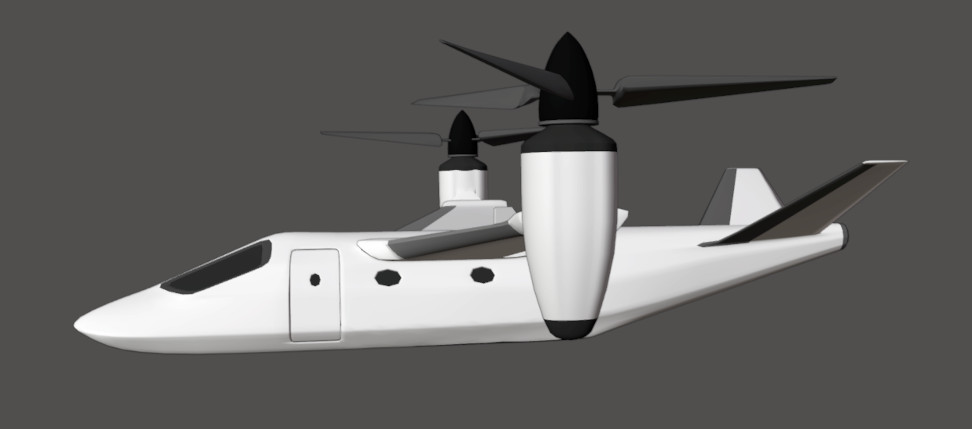
\includegraphics[width=\textwidth]{figures/tiltrotor_mesh}
    \caption[Default tiltrotor mesh]{
        The tiltrotor mesh that is provided for the \ci{Vtol} simulation mode in VTOL-AirSim.}%
    \label{fig:tiltrotor_mesh}
\end{figure}

Before we teach how to create a custom mesh, we wish to reiterate that the mesh of a vehicle is separate from the aircraft's actual dynamic model. It is simply a visual representation of the aircraft, which may or may not be an accurate representation of the vehicle's dynamics, current kinematic state, control outputs, etc. It is up to the developer to decide how the underlying model should affect the mesh, and to do the necessary work for accomplishing that. Customizing the mesh of a vehicle is a rather complicated and laborious task, even for simple cases. Therefore, you should first consider whether the needs of your project do indeed require a custom aircraft mesh or whether changing the model of the aircraft --- i.e., parameters such as mass, aerodynamic coefficients, the placement of motors, etc. --- would be sufficient. If you only need to change the model, see the VTOL-AirSim GitHub repo for instructions on how to do that.

% If you only need to change the model, see Appendix~\ref{apdx:add_configuration} for instructions on how to get started.

\subsection{Obtain a Mesh from the Internet}
Modifying the geometry of a mesh is not a straightforward process. We therefore recommend seeking online for a mesh that fits your project well and requires the least amount of modifications as possible. There is a large and ever-growing number of 3D meshes available on the internet which have been created and shared by other people. In the vast majority of cases, obtaining an off-the-shelf mesh that works for your use case will save you a considerable amount of time and effort.

One place to look for downloadable meshes is the official Unreal Engine Marketplace. With this option, you will receive Unreal asset files can be placed directly into an Unreal Project. However, because downloading a mesh from the Unreal Marketplace into an Unreal Project requires using the Epic Games Launcher --- an app only available for Windows or MacOS --- we recommend looking at third-party 3D model sharing websites first (see Chapter~\ref{chp:custom_envs} for instructions on obtaining assets from the UE Marketplace). A few examples of websites for sharing 3D meshes include \url{turbosquid.com}, \url{cgtrader.com}, and \url{sketchfab.com}. These and other similar websites contain large databases of meshes made by other people that you can download. You can explore their selections by entering search terms on their website or by viewing categories such as \textit{Aircraft} or \textit{Vehicles}.

Many of the meshes hosted on these websites are not free; nevertheless, the cost is modest compared to the time required to create one from scratch, so do not let the price steer you away from a mesh if it fits well with the requirements of your project.

As you search for an appropriate mesh, there are two things you will want to look out for: the number of polygons (also called \textit{triangles}) and the file types offered. A very high number of polygons in the mesh could cause performance issues, which might manifest itself as slowing down interactions with the Unreal Editor, or possibly slowing performance in the simulation itself. What constitutes a ``very high number'' is entirely dependent on the computer hardware in question, whether it be your machine, or the machines of others; for instance, consider those who will be working with the mesh, or those who might run simulations containing the mesh. A good rule of thumb could be to look for meshes that have less than 200,000 polygons; though that is by no means a strict limit. For a point of reference, we have tested a mesh that consisted of 440,000 polygons in a VTOL-AirSim simulation that was handled well by some machines, but on other machines it resulted in performance lags and long loading times.

Lastly, try to find a mesh that is offered in \ci{.blend} format for use with the 3D modeling software Blender. This is because nearly all meshes will require some adjustments before they can be properly used in Unreal Engine. If the mesh you find is not offered as Blender project files, you can also download the mesh in a file format that can be imported into Blender, but the import process is not guaranteed to produce a clean result.

For a mesh to be imported into UE4, it must be in FBX format. Thus, there is a possibility that you could be successful in importing a mesh directly into UE4 as an FBX file. However, in our experience, this has resulted in problems such as meshes oriented in the wrong direction, or that the axis of rotation is oriented or positioned incorrectly when animating parts of the mesh --- for example, when animating the tilt of the rotors. We therefore recommend that you open the mesh in Blender first, then export the mesh to an FBX file.

\subsection{Creating a Mesh With CAD Software}
It is also possible to create a mesh from the ground up using CAD software. If you do choose to go this route, you will still need to import the mesh into Blender in order to export it in FBX format. One way to accomplish this is to export the mesh from the CAD program as a \ci{.wrl} file (also known as VRML, or Virtual Reality Modeling Language file format), then import the resulting \ci{.wrl} file into Blender, then export from Blender to FBX format. For an example of a mesh that was created in SolidWorks and was successfully brought into UE4 using this process, see the Maker aircraft files on the MAGICC Lab's Box storage at \url{https://byu.box.com/v/magicc-maker}.

\section{Edit a Mesh in Blender}\label{sec:blender_example}

We will now walk through an example of how to take a mesh obtained from the internet and get it to fly in VTOL-AirSim. For this example, we downloaded a free mesh of a tiltrotor aircraft from \url{turbosquid.com} and placed it in the MAGICC Lab Box storage. It is available for download at \url{https://byu.box.com/v/magicc-airsim-example-mesh}. Download this ZIP file and extract it to somewhere on your machine. Note that beyond this point you will need to have Blender installed.

After extracting the ZIP file, navigate to inside of the \ci{convertiplane} folder. The contents that you see are exactly as they appeared when the mesh was first downloaded, and the files are unmodified from the originals. The actual mesh is contained in the \ci{convertiplane.blend} file. Create a copy of this file and name it \ci{aircraft.blend}. Assuming that you have already installed Blender on your machine, start Blender and open \ci{aircraft.blend}.

At the top of the window, you will notice a number of tabs with names such as \textbf{3D View Full}, \textbf{Animation}, \textbf{Compositing}, \textbf{Default}, and others. These are called \textit{workspaces}. Let's create a new workspace of type \textit{Layout}. Click the plus icon to create a new workspace and select \textbf{General > Layout}.

\subsection{Delete Unnecessary Objects}
Let's delete objects from this mesh that are not needed. In the top-right is the \textbf{Outliner} panel that lists all the objects in the scene and their hierarchies. Find the \ci{convertoplan} (\textit{sic}) object and click the arrow to the left of its name to expand it. Next, expand the \ci{b3} object that is nested inside of \ci{convertoplan}. Hold the Shift key and select \ci{b3} and everything inside \ci{b3}, then press Delete. Repeat this for all of the objects in \ci{Collection 5}, \ci{Collection 14}, and \ci{Collection 15}. After removing these objects, you should have a screen similar to Fig.~\ref{fig:blender_begin}.

\begin{figure}[t]
    \centering
    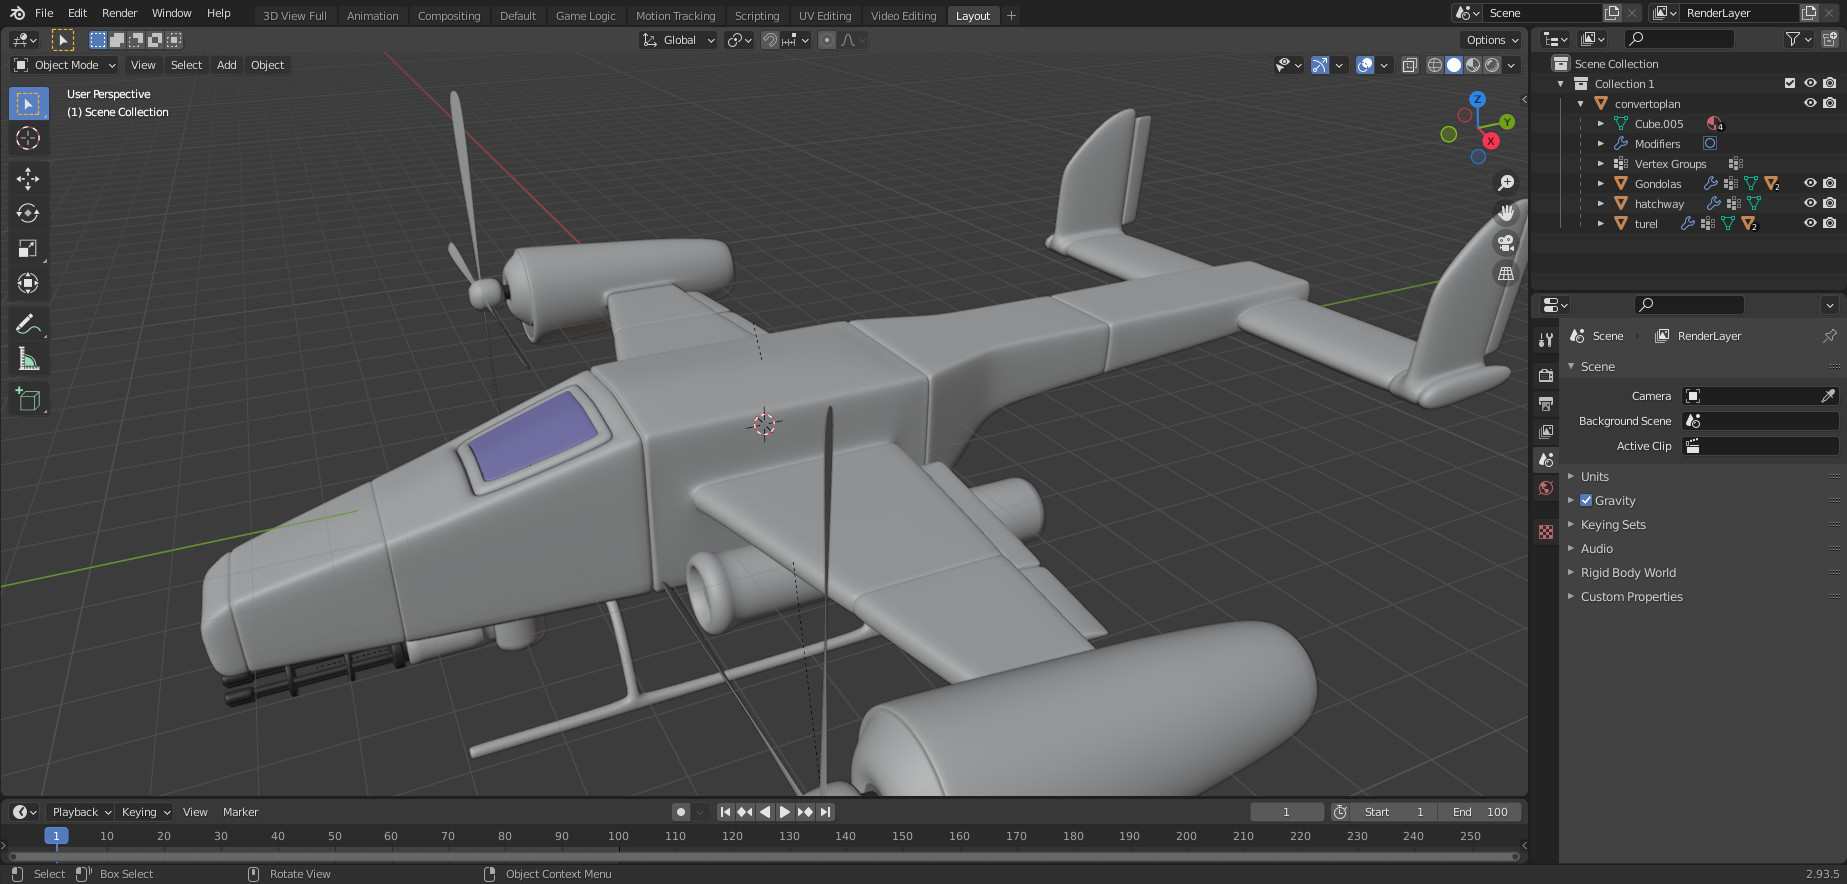
\includegraphics[width=\textwidth]{figures/blender_begin_alt}
    \caption[Blender screen of example VTOL mesh]{
        The example VTOL mesh open in Blender after removing unneeded objects.}%
    \label{fig:blender_begin}
\end{figure}

\subsection{Set the Zero Configuration}
We want forward for the aircraft to point in the +X (positive X) direction for importing into UE4. Click on the \ci{convertoplan} object to select it. Find the bottom-right \textbf{Properties} panel located directly underneath the \textbf{Outliner} and click the orange square icon to open \textbf{Object Properties}. Change each of the X, Y, and Z Location values to 0, and change the Rotation Z value to 90. Next, move your mouse over to the \textbf{Viewport} area, which is the panel currently displaying the mesh. Press the \texttt{A} key to select all objects. Press the key combination \texttt{Ctrl+A}, then click \textbf{Rotation} from the pop-up menu to apply the new rotation.

Now click on the \ci{Gondolas} object. We will refer to these cylindrical meshes as the \textit{engines}. In UE4, we will animate tilting the propellers by tilting the engines, which the propellers will follow. We want the zero rotation of the engines to be vertical, as this is what VTOL-AirSim expects. With \ci{Gondolas} selected, change the Rotation Y value to -90 and press \texttt{Enter}. Again, apply the rotation: mouse over to the \textbf{Viewport} area, press \texttt{Ctrl+A}, then click \textbf{Rotation} from the pop-up menu.

\subsection{Edit the Engines}
Select the \ci{Gondolas} object again. Notice that the two engines are a single object in Blender; we will need independent control of the tilt of each engine, so let's split the engines into two objects. In the upper-left of the \textbf{Viewport}, click \textbf{Object Mode} and select \textbf{Edit Mode}. You should now be able to see all the vertices, represented as black points, that make up the mesh of the engines. For the next part, let's move to a back view of the aircraft: in the upper-right of the \textbf{Viewport}, look for a graphic showing the global axes in red, green, and blue, and click on the hollow red circle (labeled \textbf{-X} when the holding the pointer over it). Also in the upper-right of the \textbf{Viewport} is an icon with two squares named \textbf{Toggle X-Ray}; click this icon to allow seeing all the vertices simultaneously. We can choose to separate either of the engines, so let's arbitrarily choose to separate the right engine. Draw a box around all the vertices of the right engine. You should now have a screen similar to Fig.~\ref{fig:blender_vertices} where all the vertices of the right engine are highlighted orange. Make sure your mouse is over the \textbf{Viewport} area, press \texttt{P}, then click \textbf{Selection} from the pop-up to create a new object. Change from \textbf{Edit Mode} back to \textbf{Object Mode} and click \textbf{Toggle X-Ray} to turn it off.

\begin{figure}[t]
    \centering
    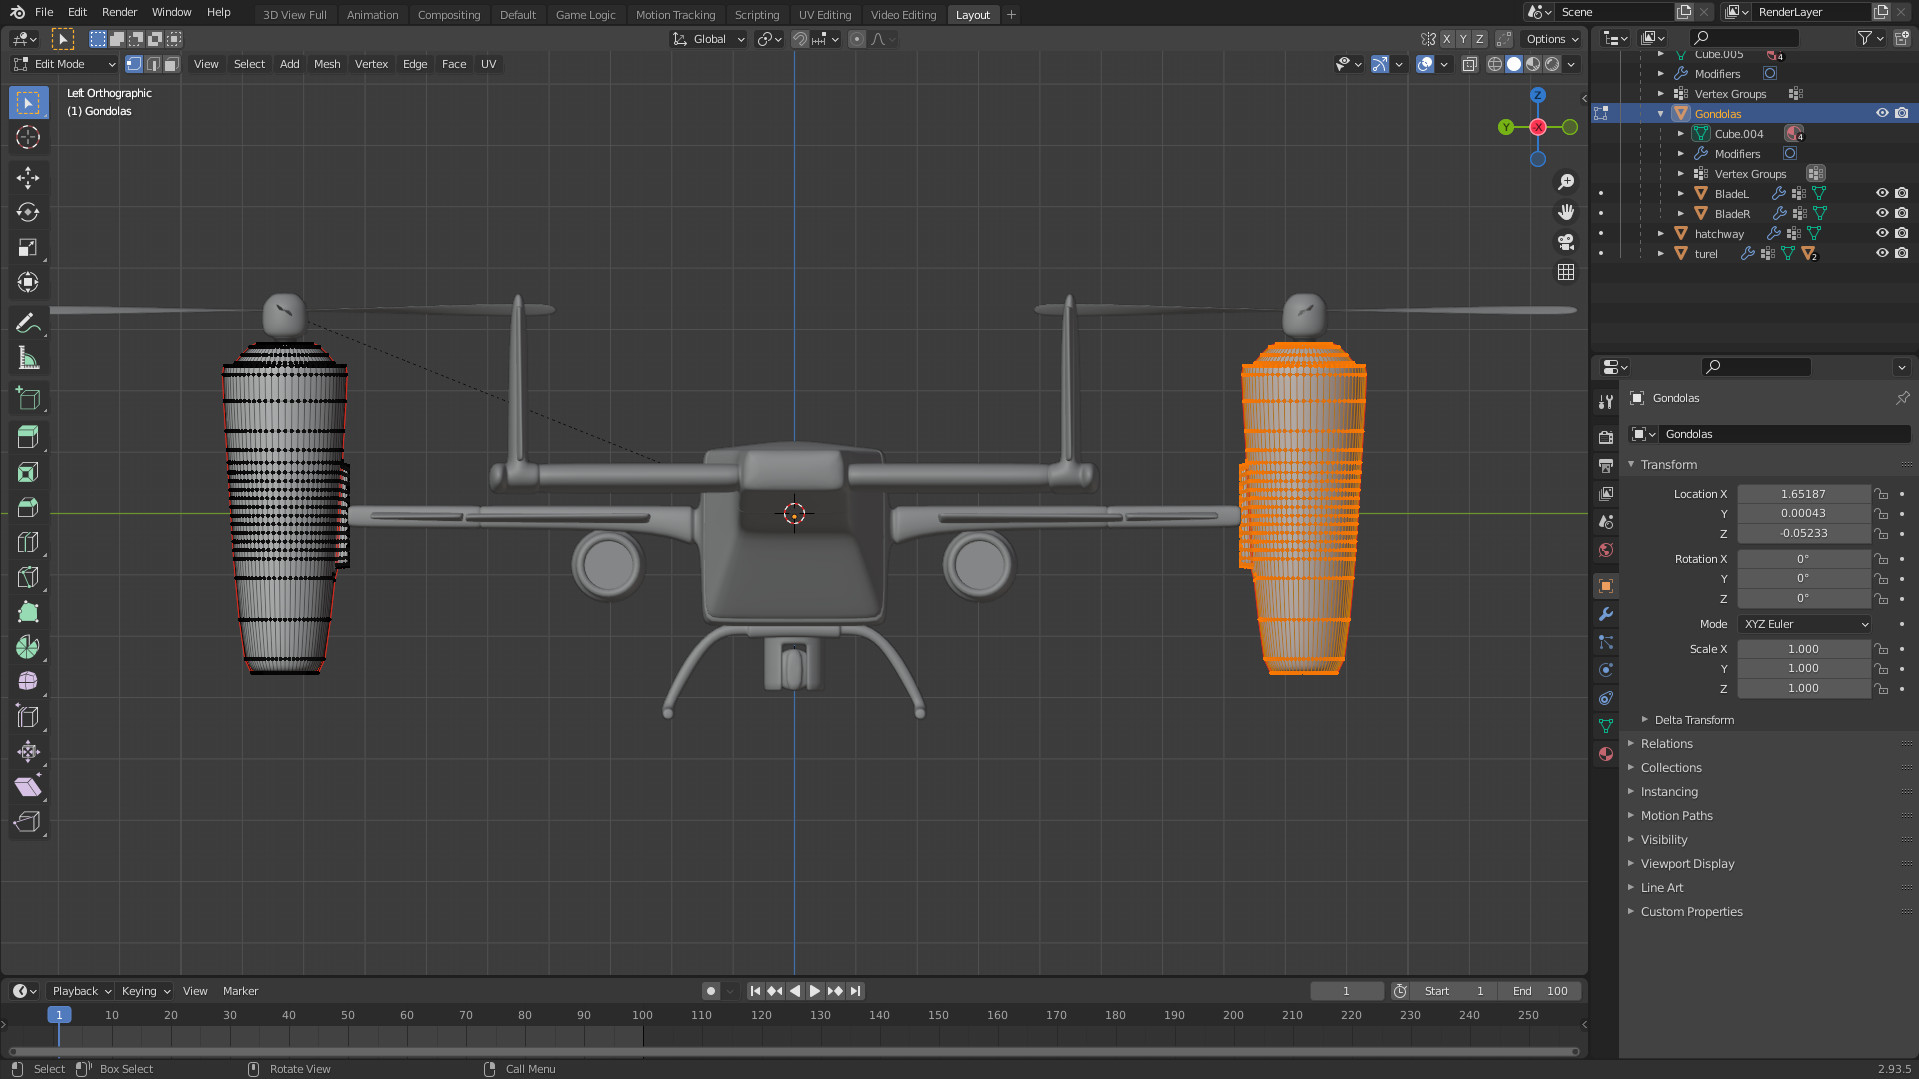
\includegraphics[width=\textwidth]{figures/blender_highlight_vertices}
    \caption[Blender screen of highlighted vertices]{
        This is how the screen should look in Blender after selecting the right engine's vertices.}%
    \label{fig:blender_vertices}
\end{figure}

In the \textbf{Outliner}, you should see an object named \ci{Gondolas} and a new object named \ci{Gondolas.001}. Rename \ci{Gondolas} to \ci{GondolaL} and \ci{Gondolas.001} to \ci{GondolaR}. Expand both \ci{GondolaL/R} objects, and find the \ci{BladeL/R} objects under \ci{GondolaL}. Click and drag \ci{BladeR}, then, while dragging, begin pressing \texttt{Shift+Alt}, and finally drop it onto \ci{GondolaR}. Doing this \textit{reparents} \ci{BladeR} to \ci{GondolaR}. Next, click and drag \ci{GondolaL}, then again press \texttt{Shift+Alt} while dragging, but this time drop it onto \ci{Collection 1}. Repeat this process for \ci{GondolaR}. This will clear their parent, which is needed to avoid a problem that occurs with nested hierarchies when exporting to FBX format.

\subsection{Move Origins of the Propellers}\label{sec:origins_props}
Next, we will fix the origins of the propellers. These origins will become the pivot points in UE4. Hold the \texttt{Ctrl} key and, in the \textbf{Outliner}, select \ci{BladeL} and \ci{BladeR}. In the top-left of the \textbf{Viewport}, click \textbf{Object} to reveal the \textbf{Object Menu}. Select \textbf{Set Origin > Origin to Geometry}. Let's also reset the zero rotations for all objects as their current rotations: hold your pointer over the \textbf{Viewport}, press \texttt{A} to select all objects, press \texttt{Ctrl+A} then click \textbf{Rotation}.

\subsection{Fix Object Names}
Finally, let's fix some object names. Rename \ci{convertoplan} to \ci{body}. With \ci{body} expanded, you will see an \textit{Object Data} item with a green triangle mesh icon named \ci{Cube.005}. Give it the same name of \ci{body}. Now do the same for the Object Data items under \ci{GondolaL}, \ci{GondolaR}, \ci{BladeL}, and \ci{BladeR} by renaming them to \ci{GondolaL}, \ci{GondolaR}, etc., respectively. Make sure each object is expanded in order to see its Object Data item. After finishing, press \texttt{Ctrl+S} to save the file.

\subsection{Export to FBX}
The mesh is ready for export. Go to \textbf{File > Export > FBX (.fbx)} to open the exporting utility window. On the right column of the window is a list of options. Under \textbf{Include} and \textbf{Object Types}, hold \texttt{Shift} and click \textbf{Mesh} and \textbf{Other}. Under \textbf{Transform} and \textbf{Up}, change the value to \textbf{Z Up}. Uncheck the option \textbf{Use Space Transform}, and check the box for \textbf{Apply Transform}. Next, expand the \textbf{Geometry} section and set \textbf{Smoothing} to \textbf{Face}. After that, you should have the settings shown in Fig.~\ref{fig:blender_fbx_export}. Finally, keep the file name as \ci{aircraft.fbx} and click \textbf{Export FBX}.

\begin{figure}[t]
    \centering
    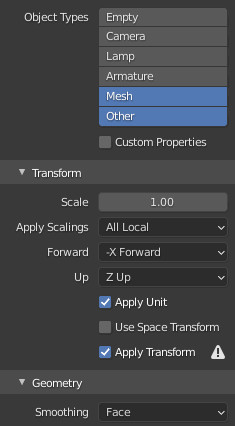
\includegraphics[height=230pt]{figures/blender_fbx_export}
    \caption[The required FBX export settings in Blender]{
        These are the required settings when exporting to FBX from Blender.}%
    \label{fig:blender_fbx_export}
\end{figure}

\section{Import Mesh Into UE4}\label{sec:import_mesh_ue4}
Once you have an FBX file of the mesh, it is time to import it into a project using Unreal Editor. In this section, we will import the mesh that we exported from Blender in the previous section. To make the instructions easier to follow, let's give a simple, memorable name to the aircraft: Homer, after the ancient Greek poet.

We will begin by creating a new Unreal Project that we can modify for this extended example by making a copy of the Blocks project. Navigate to where you have the Blocks project on your file system and create a simple copy named \ci{Blocks_test}. We want UE4 to rebuild the project, so we need to delete the \ci{Binaries}, \ci{Intermediate}, and \ci{Saved} folders in both the \ci{Blocks_test} and the \ci{Blocks_test/Plugins/vtol-AirSim} folders. The \ci{vtol-AirSim} folder also has a script named \ci{clean.sh} that you can use to automate the removal.

Start Unreal Editor and open the newly created project. To open it, do the following: if Unreal Editor is showing you the \textbf{Unreal Project Browser} window, click \textbf{More} and then \textbf{Browse}; else, if you already have a project opened, go to \textbf{File > Open Project} and then click \textbf{Browse}. Navigate to the \ci{Blocks_test} project and double-click on the file \ci{Blocks.uproject}. In the dialog that appears asking if you would like to rebuild the missing modules of Blocks and AirSim, click \textbf{Yes}.

Once the Blocks\_test project is opened, look at the \textbf{Content Browser} and ensure that \textbf{View Options > Show Plugin Content} is checked. In addition, show the \textbf{Sources panel} by clicking the icon to the left of the \textbf{Filters} icon. Now look at the \textbf{Sources panel} and navigate to \ci{AirSim Content/VTOL}. Create a folder here for the new aircraft by pressing \texttt{Ctrl+Shift+N}. Name the folder \ci{Homer}. Move inside the \ci{Homer} folder and create two new folders named \ci{Meshes} and \ci{Blueprints}.

Next, let's import the mesh. Go to \textbf{File > Import Into Level}. In the file browser dialog, find the \ci{aircraft.fbx} file that you exported from Blender earlier. In the next dialog, choose the import location as \ci{AirSim Content/VTOL/Homer/Meshes}. The next dialog will show a number of options. Under \textbf{Import Options}, check the boxes for \textbf{Import as Dynamic} and \textbf{Force Front XAxis}, then click \textbf{Import}.

A new editor window will open titled \textbf{FbxScene\_aircraft}. We will discuss this window in the the next section, so for now, return to the main Unreal Editor window. You should see the \ci{Meshes} folder populated with a number of assets. Note that these new assets are of four types: \textit{Material}, \textit{Static Mesh}, \textit{Blueprint Class}, and \textit{Fbx Scene Import Data}. The type of each asset is indicated by a colored accent along the bottom of the asset's thumbnail: green for Material, cyan for Static Mesh, blue for Blueprint Class, and purple for Fbx Scene Import Data. You can also hover your mouse pointer over any asset and the pop-up that appears will display the asset's name followed by its asset type in parentheses; for example, if you hover over the \ci{body_001} asset, it will display the title \textit{body\_001 (Static Mesh)}.

The various materials and the component meshes for the tiltrotor aircraft were originally defined in Blender, and Blender exported data about the parts and materials of the mesh into FBX format.  When Unreal Editor imported the FBX file, it tried to interpret the data and create assets that represent what is contained in the data. This process isn't perfect, and you may find that there are discrepancies between what is you can see in the scene in Blender compared with what is generated in UE4 by importing the FBX file. In this example, we won't import any textures; however, in general, you can also import the texture files supplied for a mesh (in the form of image files) separately and apply them in UE4. An easy way to change the look of the aircraft is by making simple modifications to the materials, such as color, roughness, or how metallic they look. UE4 comes with its own Material Editor, so this method allows for changing the look of the aircraft mesh inside Unreal Editor rather than requiring external tools for editing.

% You now have the tiltrotor mesh assets in your project, but they are not yet ready to be used in a simulation. While you could drag and drop any of the Static Mesh components into your level to become StaticMeshActors, without any \CC code or Blueprints (explained in the next section, Section~\ref{sec:blueprint}) to tell those Actors what to do, they will be nothing more than static props in the scene. Try this experiment for yourself, then continue to the next section to learn how we can actually use a custom mesh in a VTOL-AirSim simulation.

\section{Make a Custom Blueprint}\label{sec:blueprint}
In Unreal Engine, \textit{Blueprints} is a visual scripting system that is used to accomplish a broad range of tasks. It is a way to do visual programming in that virtually anything that the UE4 \CC libraries can do can be done using Blueprints, and vice versa. Nevertheless, some things are more easily done in Blueprints, while others are more easily done in \CC code. If you are familiar with the \textit{LabView} visual programming system from National Instruments, they share some similarities. For our purposes of creating a controllable aircraft, you can also think of it as having similarities with what are called \textit{assemblies} in some CAD software. In addition, a Blueprint is interchangeably called a \textit{Blueprint Class} because it is a class in the same sense of the word's meaning in \CCd. You create an \textit{instance} of a Blueprint Class by spawning or placing an Actor in the level of that Blueprint Class. As an example, there is one \ci{TiltrotorPawn} \CC class and one \ci{BP_TiltrotorPawn} Blueprint for the tiltrotor vehicle, but we can spawn one or more tiltrotor vehicles in a simulation where each one has a different name, a different state, etc.

While almost everything in VTOL-AirSim is contained in the \CC code, a few aspects concerning the mesh animation is contained in the form of Blueprints. In particular, this includes:
\begin{itemize}
    \item The Static Meshes that are used to visually represent the aircraft
    \item The relationships between the meshes (i.e., the hierarchies and relative transforms)
    \item The mechanism which sets the rotation speed of the propellers
    \item The Materials assigned to each Material Slot
\end{itemize}

\subsection{Notes on Naming Conventions}
First, we wish to cover a few definitions and naming conventions. A \textit{Pawn} in Unreal Engine is defined as ``the base class of all Actors than can be controlled by players or AI''. All of the aircraft in VTOL-AirSim are derived classes of the Pawn \CC class, and thus have the naming convention of appending \textit{Pawn} to the class name. Each vehicle mesh consists of a Blueprint that inherits from one of the vehicle Pawn \CC classes. A Blueprint for a vehicle mesh has the prefix \textit{BP\_}, and this is how AirSim's multirotor vehicle and VTOL-AirSim's tiltrotor got the names \ci{BP_FlyingPawn} and \ci{BP_TiltrotorPawn}, respectively.

\subsection{Relative Transforms in Blueprints}
Section~\ref{sec:import_mesh_ue4} had you use the \textbf{Import Into Level} feature, and this tries to automatically create a Blueprint based on the data contained in the FBX file. This is the \textbf{FbxScene\_aircraft} Blueprint. Go back to the editor window for the Blueprint, or double-click on the asset in the \textbf{Content Browser} if you no longer have the window. In the Blueprint editor, switch to the \textbf{Viewport} tab. On the left of the window, you will see the \textbf{Components} panel which contains a hierarchy of \textit{Components} which make up the Blueprint that reflects the same hierarchy of objects that we saw in Blender. Click on the \ci{GondolaR} Static Mesh Component, then look at the \textbf{Details} panel on the right side of the window. Notice that its Location X, Y, and Z values reflect their values set in Blender, except that the Y-axis is negated and they are all multiplied by 100 --- this is because UE4 uses a left-handed North-East-Up coordinate system, and its base unit of length is the centimeter (Blender is unitless by default, but UE4's process of interpreting the FBX specification causes the values to be multiplied by 100, which is desirable in this case). However, you will see that the same is not true for \ci{BladeR}; the values are a bit different than in Blender. This is because in Blender the Location values are relative to the global coordinate frame (assuming that the Location transform has not been applied), while in UE4, the Location values are relative to the coordinate frame of its \textit{parent}, which in this case is \ci{GondolaR}.

\subsection{Origins (Pivot Points) of Meshes}
Understanding where the origin of a mesh (or \textit{pivot point}, as it is called in Unreal Engine) comes from is very important, because \textit{there is no way to change the origin (pivot point) of a mesh in Unreal Engine}. The pivot point of each Static Mesh is read by UE4 at the time of import and then becomes fixed, both its position and orientation, after the asset is generated. This is why we set the origins of the propeller objects to be at their geometric centers in Section~\ref{sec:origins_props}, as it is only in Blender (or some other 3D modeling software) that the position of the point can be changed, as well as the orientation of the coordinate axes with respect to the mesh. If you are having problems getting the right pivot points for meshes, see Appendix~\ref{apdx:blender_origins_alt} for an alternate method of correcting origins in Blender.

\subsection{Create a New Blueprint}
Each unique vehicle must have its own Blueprint to fly in VTOL-AirSim. We could modify the \ci{FbxScene_aircraft} Blueprint that UE4 created for us, but this would require more work than modifying a copy of the \ci{BP_TiltrotorPawn} Blueprint, so we will do the latter.

Copying a Blueprint must be done in Unreal Editor. In the \textbf{Content Browser}, navigate to the folder \ci{AirSim Content/VTOL/Tiltrotor/Blueprints}. With the \textbf{Sources panel} open, click and drag the \ci{BP_TiltrotorPawn} asset to the \textbf{Sources panel} and drop it onto the \ci{VTOL/Homer/Blueprints} folder, then select \textbf{Copy here} from the pop-up. Navigate to that same folder and rename the copied Blueprint to \ci{BP_HomerPawn}, then double-click it to open the Blueprint Editor. Click on the \textbf{Viewport} tab in the Blueprint Editor so you can see the changes we will make in the next steps.

\subsection{Replace the Static Mesh Components}
At this point, you should see the default tiltrotor aircraft in VTOL-AirSim. Let's replace the Static Mesh Components in the Blueprint with the new aircraft mesh. Select all the Static Mesh Components under the \ci{Body} component by holding \texttt{Shift} while clicking on them, and press \texttt{Delete} to remove them. Next, click on the \ci{Body} component and find the \textbf{Static Mesh} property in the \textbf{Details} panel. To change it, click on the mesh name to reveal a drop-down list, begin typing \texttt{body}, and then select \ci{body_001} (or similarly named) from the filtered list. Now you should see the body of the new aircraft in the \textbf{Viewport}; the Static Mesh of the \ci{Body} Static Mesh Component (which is the Blueprint's Root Component) has now been set to the body of the new aircraft mesh.

\begin{figure}[t]
    \centering
    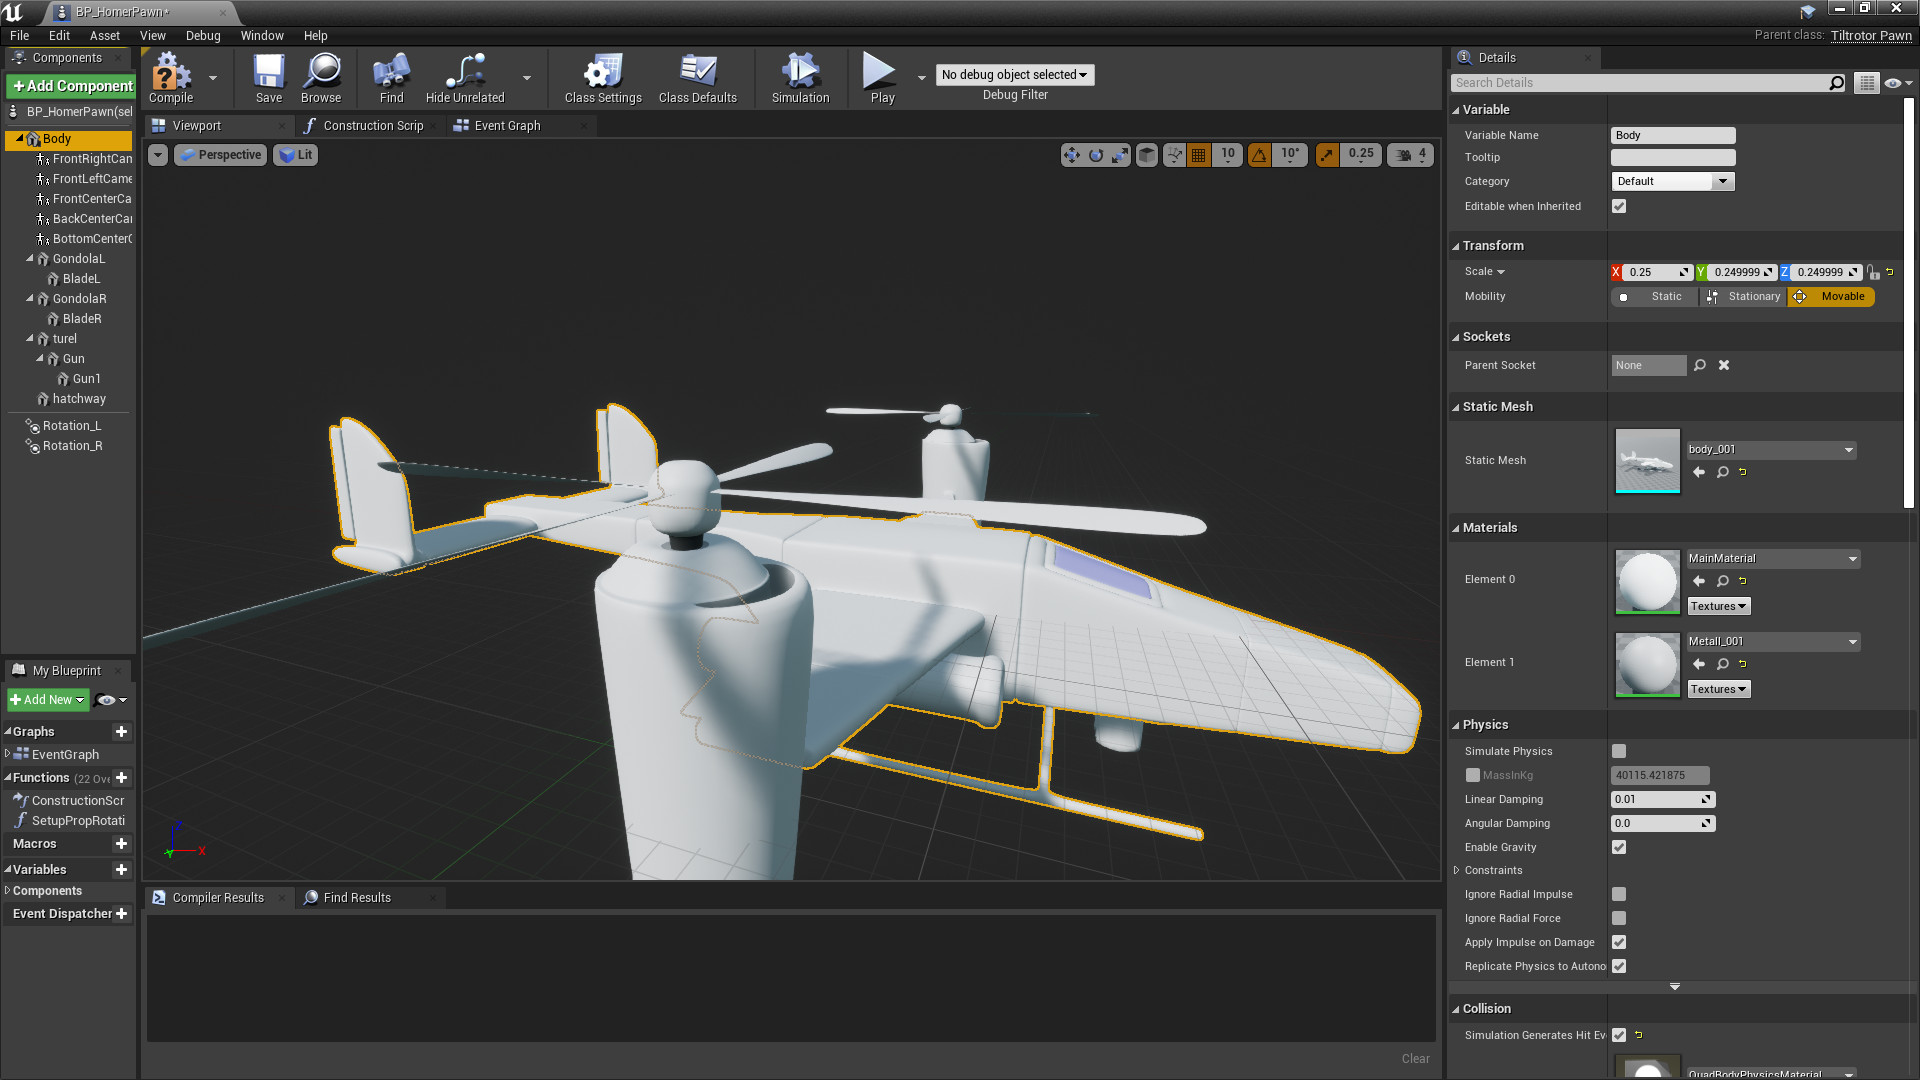
\includegraphics[width=\textwidth]{figures/ue4_blueprint_viewport}
    \caption[Viewport of Blueprint with example aircraft mesh]{
        The Viewport of \ci{BP_HomerPawn} after adding all of the new aircraft's Static Mesh Components to the Blueprint.}%
    \label{fig:ue4_blueprint_viewport}
\end{figure}

The next task is to copy the configuration of the Static Mesh Components contained in the \ci{FbxScene_aircraft} Blueprint to the \ci{BP_HomerPawn} Blueprint. Select all the Static Mesh Components in \ci{FbxScene_aircraft} using \texttt{Shift} and click, then right-click on any of the selected components and select \textbf{Copy}. In the editor for \ci{BP_HomerPawn}, right-click on \ci{Body} and select \textbf{Paste}. Finally, delete the \ci{body1} component from the components that you just pasted. You should now see the full aircraft mesh in the \ci{BP_HomerPawn} Viewport, as shown in Fig.~\ref{fig:ue4_blueprint_viewport}.

\subsection{Edit \texttt{SetupPropRotationMovement}}\label{sec:ue4_blueprint_setupprop}

There is one visual programming piece of the Blueprint that needs to be edited. In the \textbf{My Blueprint} panel located in the lower-left of the window, under the \textbf{Functions} section, find the function named \ci{SetupPropRotationMovement} and double-click it to open it in a new tab. Notice the two boxes titled \textbf{Set Updated Component} where the left and right boxes have connections to nodes labeled \textbf{Rotation L} and \textbf{Rotation R}, respectively. Hold your mouse pointer over the \textbf{Rotation L} node --- but not its label, rather over the empty space to the left of the label text --- and the tooltip tells you \textit{Read the value of variable Rotation\_L}. Indeed, this and the \textbf{Rotation R} node read the values from the \ci{Rotation_L} and \ci{Rotation_R} Rotating Movement Components of this Blueprint (see the \textbf{Components} panel) and feed those values as inputs to the \textbf{Set Updated Component} functions.

\begin{figure}[ht]
    \centering
    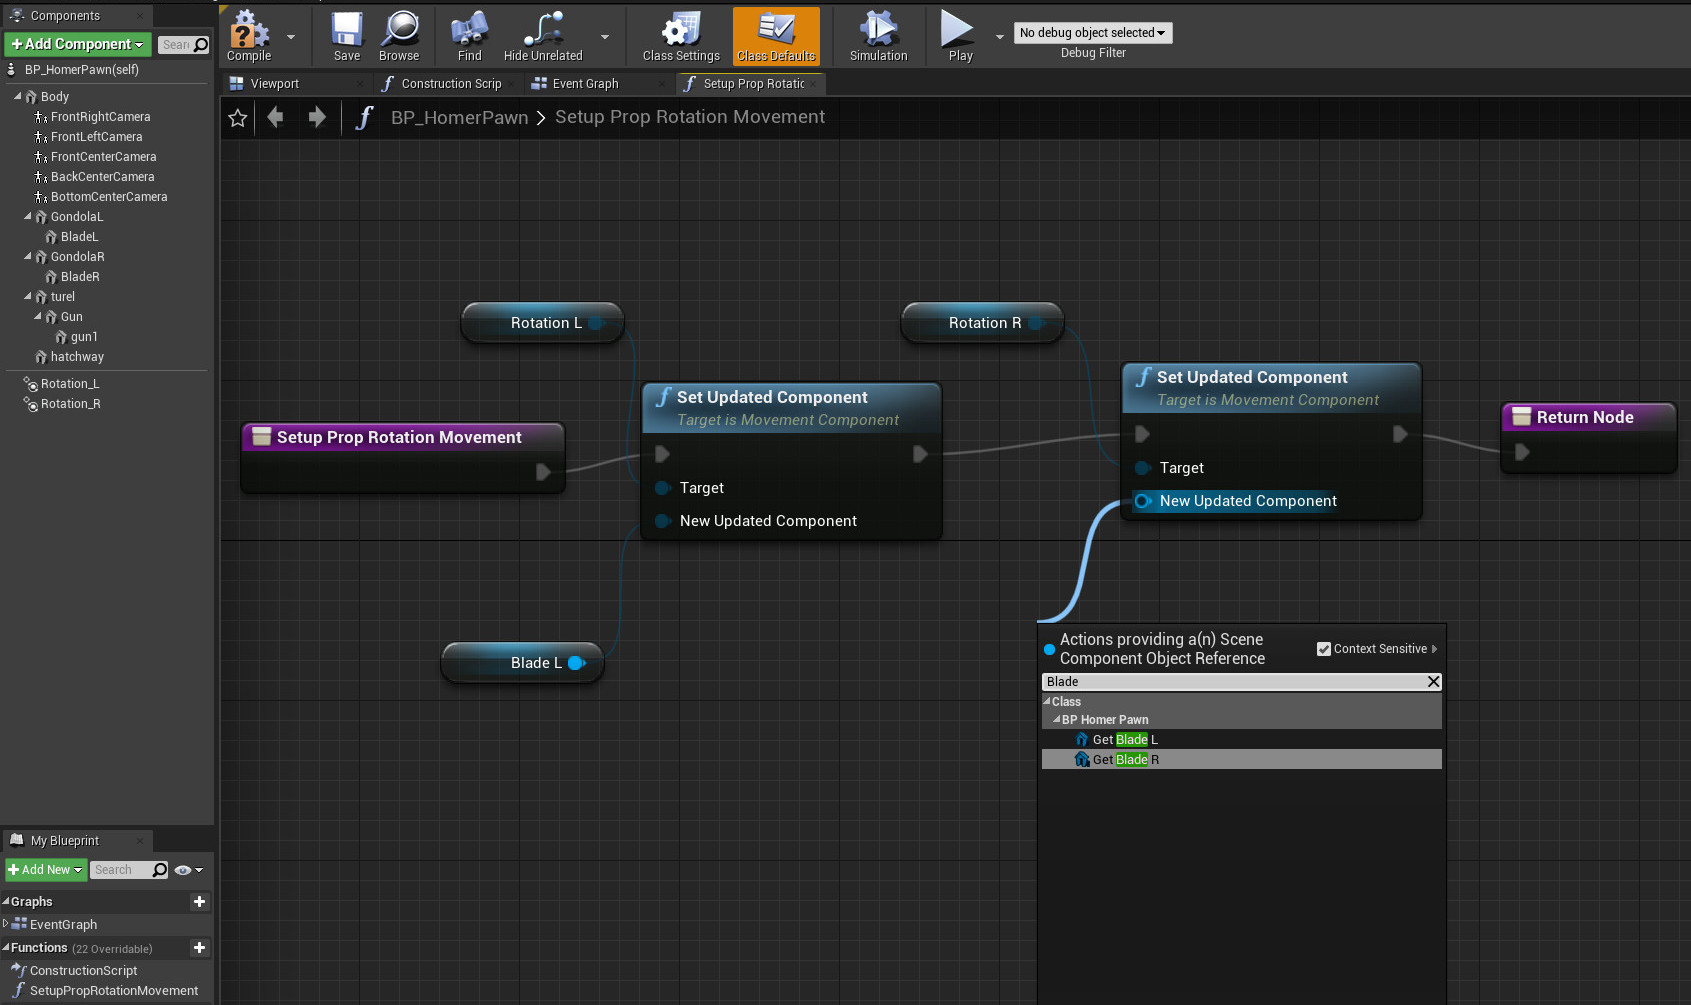
\includegraphics[width=\textwidth]{figures/ue4_blueprint_setupproprotation2}
    \caption[Editing the Blueprint function SetupPropRotationMovement]{
        In the \ci{SetupPropRotationMovement} function, what appears after clicking on the \textbf{New Updated Component} terminal, dragging outward, releasing, and then typing the search term \texttt{Blade}.}%
    \label{fig:ue4_blueprint_setupproprotation}
\end{figure}

If you look at the same function in \ci{BP_TiltrotorPawn}, you will see that the each box also has output connections going to nodes labeled \textbf{Prop L} and \textbf{Prop R}, which correspond to the \ci{Prop_L} and \ci{Prop_R} components of the Blueprint; these nodes and connections were present when we first copied the \ci{BP_TiltrotorPawn} Blueprint, but the nodes were deleted when we deleted the \ci{Prop_L/R} components.

What this function does is it links together the \textit{Rotating Movement Components} in the Blueprint to the Static Mesh Components that we want to animate. In UE4, a Rotating Movement Component is a non-scene component (i.e., it is not rendered and has no position) which simply ``performs continuous rotation of a component at a specific rotation rate''. AirSim uses Rotating Movement Components in order to set the speed that the propellers rotate. In the \CC code, it is the \ci{RotationRate.Yaw} of the Rotating Movement Components that get set by their calculated values based on control inputs in AirLib, and it is in this Blueprint function where each of the \ci{Rotation_L/R} components are linked to affect each of the propellers.

In \ci{BP_HomerPawn}, we simply need to have \ci{BladeL/R} be the outputs of the left and right boxes. To create output connections to new nodes for these boxes, click on the terminal (the hollow circle) of \textbf{New Updated Component} and drag downward toward any empty area and release; this will reveal a pop-up which allows you to search for the node you want to create (see Fig.~\ref{fig:ue4_blueprint_setupproprotation}). Type \texttt{Blade}, and click on \textbf{Get Blade L} for the left box, or \textbf{Get Blade R} for the right box. Follow this process for both boxes.

Once you have a connection from the \textbf{New Updated Component} terminal of the left box to \textbf{Blade L} and a connection from the right box to \textbf{Blade R}, you are finished with the Blueprint. Save your changes.

\section{Perform a Test Flight}
% We are ready to perform the first test flight of the Homer aircraft in the Unreal Editor. First, we need to tell AirSim that we have a different Blueprint than the default that we want to use. We can do this in the \ci{settings.json} file for AirSim using the \ci{PawnPaths} setting. Create a new \ci{settings.json} file at the path \ci{~/Documents/AirSim} on your machine and give it the following content:
We are ready to perform the first test flight of the Homer aircraft in the Unreal Editor. First, you will need to place the following settings in your \ci{settings.json} file:
\begin{minttcb}[title={AirSim Settings For Custom HomerPawn Aircraft}]{json}
{
  "SettingsVersion": 1.2,
  "SimMode": "Vtol",
  "PawnPaths": {
    "DefaultVtol": {
      "PawnBP":
        "Class'/AirSim/VTOL/Homer/Blueprints/BP_HomerPawn.BP_HomerPawn_C'"
    }
  },
  "Vehicles": {
    "uav0": {
      "VehicleType": "VtolSimple"
    }
  }
}
\end{minttcb}
In the \ci{PawnPaths} setting, we specify what we want to use as the default Blueprint for all vehicles of type \ci{Vtol} (this can also be configured for each vehicle, if needed) so that AirSim will choose \ci{BP_HomerPawn} rather than the default \ci{BP_TiltrotorPawn}. The somewhat confusing string that is required to specify \ci{BP_HomerPawn} is due to how UE4 deals with paths within projects as well as how UE4 generates object names. In short, the class object for \ci{BP_HomerPawn} becomes \ci{BP_HomerPawn.BP_HomerPawn_C}, contained within the single quotes is the path string to the serialized object, and the text \ci{Class} means the object is of type \ci{Class} --- other types include \ci{Material}, \ci{StaticMesh}, etc. See Appendix~\ref{apdx:unreal_paths} for an explanation of path references in UE4.

After you have saved the \ci{settings.json} file, go back to Unreal Editor. In the \textbf{World Outliner}, find the \textbf{FbxScene\_aircraft} Actor that UE4 automatically placed in your level. Select it and press \texttt{Delete}. Next, click \textbf{Play} in Unreal Editor. You should see a \ci{BP_HomerPawn} Actor spawn in the Blocks world. In a terminal, run the geometric controller example from Section~\ref{sec:vtol_geometric_control}. After running the \ci{geometric_control_airsim_sim.py} script, you should see the aircraft take off and fly until it hits a wall. Notice that the propellers are spinning as they should, but the engines never tilt. Click \textbf{Stop} to end the simulation.

There is a very simple reason as to why the engines were not tilting: the names of the engines are hard-coded as \ci{Engine_L} and \ci{Engine_R} in the \CC code, yet HomerPawn's engines are named \ci{GondolaL/R}. There are two ways in which you can solve this problem: you can fix the names of the engine components in the Blueprint, or you can create a new \CC class for the Homer aircraft which uses appropriate names. In order to demonstrate how to create a new vehicle \CC class for those who may need more advanced customizations, we are going to do the latter option. If you do not think you will need to modify any of the VTOL-AirSim code for your project, then you can do the former option and stop there. Otherwise, close out of Unreal Editor and continue to the next section.

\section{Create a \texorpdfstring{\CCh}{C++} Class}\label{sec:cpp_class}
In this section, we create a replica of the \ci{TiltrotorPawn} source code and rename it to \ci{HomerPawn}. Then, we modify the code to correctly animate the tilting of the engines on the Homer aircraft mesh.

\subsection{Copy Files from TiltrotorPawn}
First, go to \ci{Blocks_test/Plugins/vtol-AirSim/Source/Vehicles}. Create a new folder and name it \ci{Homer}. From the \ci{Tiltrotor} folder, copy the files \ci{TiltrotorPawn.h} and \ci{TiltrotorPawn.cpp} into the \ci{Homer} folder and rename them to \ci{HomerPawn.h} and \ci{HomerPawn.cpp}.

Next, open VS Code in the folder \ci{Homer}. Press the keys \texttt{Ctrl+Shift+F} to search across all files in the opened directory. Type \texttt{Tiltrotor} into the \textbf{Search} box. Click the small arrow to the left of the search box to reveal the \textbf{Replace} box. Enter \texttt{Homer} as the replacement term. Click the \textbf{Replace All} icon to the right of the \textbf{Replace} box, or press the keys \texttt{Ctrl+Alt+Enter}. Click \textbf{Replace} in the dialog that appears.

There is one class that should keep its original name --- \ci{TiltrotorPawnEvents} --- as we don't need to change anything in it to be compatible with \ci{HomerPawn}. Repeat the same process to replace occurrences of \ci{HomerPawnEvents} with \ci{TiltrotorPawnEvents}. Lastly, in \ci{HomerPawn.h}, change the include statement from \ci{"TiltrotorPawnEvents.h"} to use the correct file path of \ci{"Vehicles/Tiltrotor/TiltrotorPawnEvents.h"}. With those changes, you now have a \CC class for \ci{HomerPawn} that can compile without errors.

\subsection{Correct Names of Engine Components}
We still need to fix the names of the engine components before the class will be fully functional. In VS Code, open \ci{HomerPawn.cpp} and find the two lines containing the strings \ci{"Engine_L"} and \ci{"Engine_R"}. Change each string to be \ci{"GondolaL"} and \ci{"GondolaR"}. Notice, in addition, the lines containing the strings \ci{"Rotation_L"} and \ci{"Rotation_R"}; this is where the Rotating Movement Components that we discussed in Section~\ref{sec:ue4_blueprint_setupprop} are specified. We don't need to change those strings because the component names remain the same in \ci{BP_HomerPawn}. Note also that these two arrays of components are looped over in the function \ci{SetRotorRenderedStates} later on in the file. This is where their values are set, and they are set according to the data contained in the vector \ci{rotor_infos}, which ultimately comes from AirLib.

This completes our changes to the code. Run the script \ci{clean.sh} in \ci{vtol-AirSim} and launch Unreal Editor. Open the \ci{Blocks_test2} project and click \textbf{Yes} on the dialog to rebuild the modules.

\subsection{Reparent the Blueprint}
Once Unreal Editor has rebuilt and opened the project, open \ci{BP_HomerPawn} again to make a necessary change. In the toolbar near the top of the Blueprint Editor, click on \textbf{Class Settings}. In the \textbf{Details} panel, find the \textbf{Parent Class} field and click on the field's current value of \textbf{Tiltrotor Pawn}. Begin typing \texttt{Homer} and you should see \textbf{Homer Pawn} appear from the list of filtered items. Select \textbf{Homer Pawn}, then click \textbf{Continue} on the dialog to reparent the Blueprint. The \textbf{Homer Pawn} class is the \ci{AHomerPawn} \CC class that you created; if it shows up in the list of classes, that means UE4 successfully built your new class. Lastly, save the changes to the Blueprint.

This step of reparenting creates the actual link between the \ci{BP_HomerPawn} Blueprint and the \ci{AHomerPawn} \CC class. Now, when a \ci{BP_HomerPawn} Actor is spawned, it will use your custom code in \ci{HomerPawn.cpp}.

\section{Improve the Look With Materials}
You are now ready for a fully functional test flight of the Homer aircraft. But before we do the final flight, let's improve the look of the aircraft by changing the Materials assigned to the Material Slots of the various components. We will do that by reusing Materials from the VTOL-AirSim tiltrotor aircraft.

In the Blueprint Editor for \ci{BP_HomerPawn}, make sure the \ci{Viewport} tab is active. In the \textbf{Components} panel, select the \ci{Body} component. Find the Material Slot named \textbf{Element 0} and click on the currently selected material named \textbf{MainMaterial}. Type \texttt{body}, and select the first item with the name \textbf{body} (from the VTOL-AirSim tiltrotor assets). Repeat this for the engines \ci{GondolaL/R}, and for the \ci{hatchway} component. Do the same for each of the propellers, \ci{BladeL/R}, but instead search for and select the \textbf{blades} Material. In the \textbf{Viewport} of the Blueprint Editor, you should see the Homer aircraft with a greatly improved look.

\section{Final Test Flight}
Now let's perform the test flight. Go to the main Unreal Editor window and click \textbf{Play}. In a terminal, run the geometric controller script as before. If everything has gone well up to this point, then you should see the engines properly tilting on the Homer mesh as it takes off and flies through the Blocks world (and into a wall), as seen in Fig.~\ref{fig:homerpawn_flight}.

This completes our full custom aircraft example. In the next chapter, we show how you can create a custom environment for use with VTOL-AirSim.

\begin{figure}[h]
    \centering
    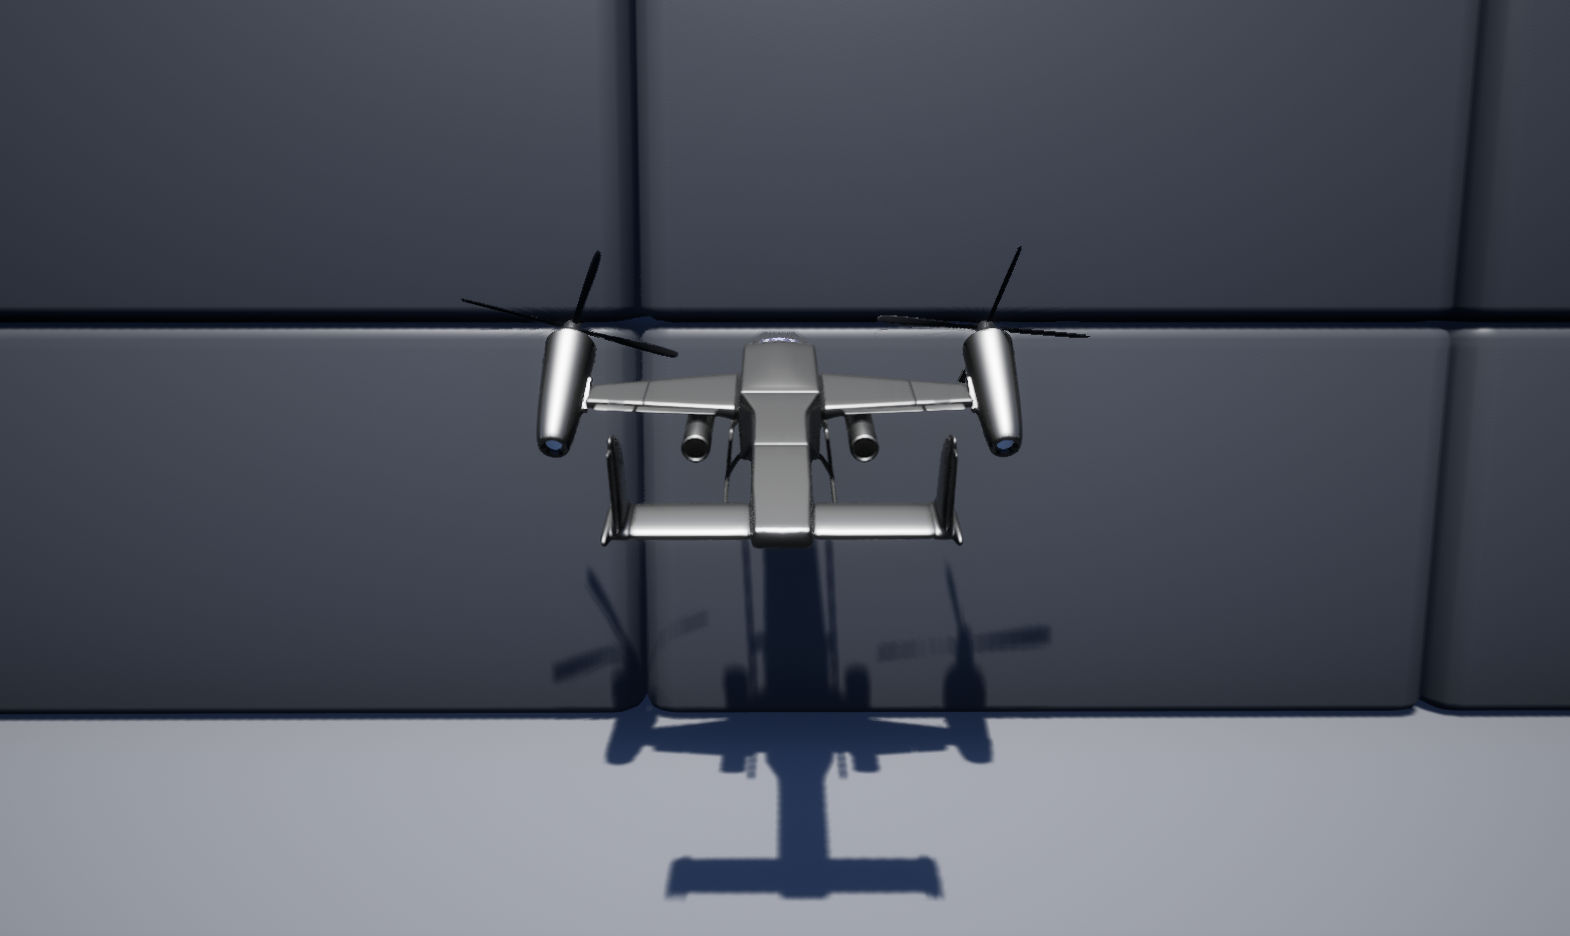
\includegraphics[width=\textwidth]{figures/homerpawn_final_flight}
    \caption[Custom aircraft flying in VTOL-AirSim]{
        The custom Homer aircraft flying in the Blocks world as it hits a wall.}%
    \label{fig:homerpawn_flight}
\end{figure}

% First, go to \ci{Blocks_test/Plugins/vtol-AirSim/Source/Vehicles}. Create a copy of the \ci{Tiltrotor} folder and name it \ci{Homer}. In \ci{Homer}, there should be eight files, where each one contains \ci{Tiltrotor} in some part of its name. Rename each file by replacing \ci{Tiltrotor} with \ci{Homer}; for example, rename the files to be \ci{HomerPawn.h}, \ci{SimModeWorldHomer.cpp}, \ci{HomerPawnEvents.h}, etc.

% Next, open VS Code in the folder \ci{Homer}. Press the keys \texttt{Ctrl+Shift+F} to search across all files in the opened directory. Type \texttt{Tiltrotor} into the \textbf{Search} box. Click the small arrow to the left of the search box to reveal the \textbf{Replace} box. Enter \texttt{Homer} as the replacement term. Click the \textbf{Replace All} icon to the right of the \textbf{Replace} box, or press the keys \texttt{Ctrl+Alt+Enter}. Click \textbf{Replace} in the dialog that appears. And with that, you now have \CC classes for \ci{HomerPawn} that can compile without errors.

% \subsection{Correct Names of Engine Components}
% Now we need to fix the names of the engine components. In VS Code, open the file \ci{HomerPawn.cpp} and find the two lines containing the strings \ci{"Engine_L"} and \ci{"Engine_R"}. Change each string to be \ci{"GondolaL"} and \ci{"GondolaR"}, respectively. Notice the two lines near it containing the strings \ci{"Rotation_L"} and \ci{"Rotation_R"}; this is also where the Rotating Movement Components that we discussed in Section~\ref{sec:ue4_blueprint_setupprop} are specified. We don't need to change those strings because the component names remain the same in \ci{BP_HomerPawn}. Note also that these two arrays of components are looped over in the function \ci{SetRotorRenderedStates} later on in the file, where their values are set by according to the data contained in the vector \ci{rotor_infos}, which ultimately comes from AirLib.



% \subsection{Add Workaround to \ci{SimHUD.cpp}}
% There is one more file that we need to change. The folder \ci{vtol-AirSim/Source/SimHUD} contains a file named \ci{SimHUD.cpp}. Open this file in VS Code. In this file, the \ci{SimMode} setting from the user's \ci{settings.json} file is read, and depending on its value, it will spawn one of the vehicle types of VTOL-AirSim; or rather, \ci{ASimModeWorldMultirotor/Tiltrotor} for the aerial vehicles.

% We need VTOL-AirSim to spawn \ci{}


% \subsubsection{When Editing or Creating a Mesh is Required}
% If for any reason you find that you must make modifications to a mesh, then you will need to use 3D modeling software to do so. We define \textit{edit a mesh} in this context to mean modifying the geometry of a mesh, the organization of its parts/components (including the hierarchy or naming of components), or the \textit{material slots} (as opposed to the actual materials, which are set in UE4) that are baked into its FBX file. For these types of tasks, we highly recommend using the free 3D modeling software Blender. See Appendix~\ref{apdx:blender} for more information about Blender. Modifying the geometry of a mesh can be a complex task and is a very broad topic, so we will not cover it in this text. To change the organization of a mesh's components or its material slots, a brief overview is given in Appendix~\ref{apdx:blender}.

\chapter{Custom Environments}\label{chp:custom_envs}
This chapter explains how to create a custom environment for use with VTOL-AirSim. Like the previous chapter on custom aircraft, this chapter is structured as a guide through a specific example that demonstrates the complete process starting with obtaining assets from the Unreal Engine Marketplace to a full VTOL-AirSim simulation in the new environment.

We begin with a discussion on obtaining assets from the Unreal Engine Marketplace. The proceeding sections are a guide through a specific example in which we first create a new Unreal Project, then we add to the project Unreal Engine assets from the marketplace, and finally we add the VTOL-AirSim Plugin.

\section{Unreal Engine Marketplace}
The easiest way to create a custom environment is by downloading a prebuilt environment from the Unreal Engine Marketplace, found at \url{https://unrealengine.com/marketplace}. In contrast to an aircraft in VTOL-AirSim, which is a small mesh made up of a few moving parts, an environment is much larger, and is typically composed of a great number of meshes and other details such as lighting, sky objects, bodies of water, and dynamic actors arranged in a complex layout. Creating an environment --- or a \textit{level}, as it is called in UE4 --- on one's own requires a deep understanding of Unreal Engine to do well. However, if you are able to obtain a level that is already made, the process is very simple.

The Unreal Engine Marketplace has a large selection of assets available to download. Many of them are paid, though there is a significant amount of free assets to choose from. The assets on the marketplace are of all types of UE4 assets, including Materials, Textures, Static Meshes, Blueprints, etc., so you must be careful in that you choose a product that contains one or more levels among the provided assets. Study the product's description to know whether it comes with a prebuilt level. As an example, the images for a product could be pictures of different types of buildings with scenic backgrounds, yet the product simply contains an assortment of buildings, without any levels containing those buildings. These are assets that are meant to be used by creators who are designing their own levels. Note that you may find levels referred to as \textit{maps} in product descriptions, due to level assets having the file extension \ci{.umap}. Also, some products do come with prebuilt levels but simply fail to mention this in their descriptions, so you can also check the \textbf{Reviews} and \textbf{Questions} tabs when viewing a product for more clues.

When searching for assets, you also need to choose assets that are compatible with the version of Unreal Engine which you are using. You can filter results while searching for assets on the UE Marketplace by clicking the label of your version in the \textbf{Filter Results} column under \textbf{Supported Engine Versions}.

\section{Obtain Assets from Unreal Engine Marketplace}\label{sec:obtain_assets_windows}
As of this writing, the only way to download assets obtained on the UE Marketplace is through the \textit{Epic Games Launcher}, and it is only available for Windows or MacOS. While it is theoretically possible to use the Epic Games Launcher on Linux using the compatibility layer \textit{Wine}, that is outside the scope of this text. The example in this chapter has only been tested using Windows, so we will provide instructions for Windows only.

The Epic Games Launcher and Unreal Engine on Windows are free software, so all you need is access to a machine, hard drive, partition, or virtual machine that has an instance of Windows for which you have internet access and admin rights to download and install software. You also need at least 40 GB of free space available in Windows.
%  for the Epic Games Launcher, Unreal Engine (about 36 GB), and the new Unreal Project you will make with new assets downloaded from the UE Marketplace.

\subsection{Install The Epic Games Launcher and Unreal Engine (Windows)}

On Windows, go to \url{https://epicgames.com/store/en-US/download} to download the Epic Games Launcher installer. Install it and open it. When it opens, it will ask you to sign in to your Epic account. Sign in using your Epic Games account (you should already have one if you've done the steps in Section~\ref{sec:unreal_requirements}). Next, click on the \textbf{Library} tab. Click the plus icon next to \textbf{Engine Versions} to install a version of Unreal Engine (Fig.~\ref{fig:egl_ue_version}). Click on the version number then select whichever version is compatible with AirSim; at the time of this writing, it is Unreal Engine version 4.25. Note that the last number in the version label, called the patch version, doesn't determine compatibility, so just choose the highest patch version, which is 4.25.4 at the time of this writing. Once you have chosen a version, click \textbf{Install}. The download and installation will take a while complete.

\begin{figure}[h]
    \centering
    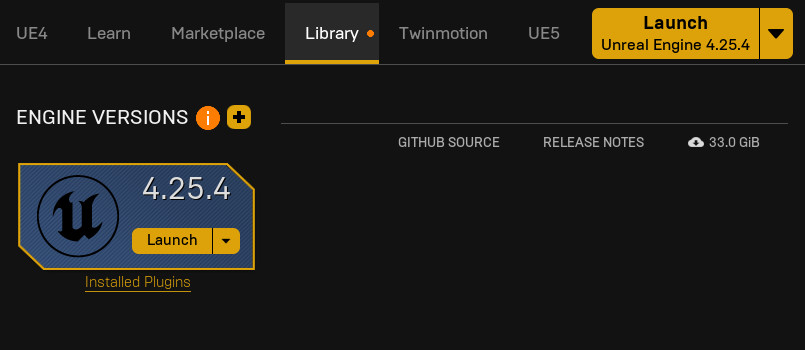
\includegraphics[width=\textwidth]{figures/egl_ue_version2.jpg}
    \caption[Epic Games Launcher: Install Unreal Engine]{
        The Epic Games Launcher with Unreal Engine 4.25.4 installed.}%
    \label{fig:egl_ue_version}
\end{figure}

\subsection{Create a New Unreal Project (Windows)}
When the installation of Unreal Engine has finished, click \textbf{Launch} to start Unreal Editor. You will be presented with a window after it initializes. Create a new project by doing the following: select \textbf{Games} and click \textbf{Next}, then select \textbf{Blank} and click \textbf{Next}, then click \textbf{With Starter Content} and change it to \textbf{No Starter Content}, and finally give it the name \ci{CoolBridge} and click \textbf{Create Project}.

\subsection{Download Assets from Marketplace (Windows)}
You can explore the UE Marketplace from either a web browser or within the Epic Games Launcher. Let's do so with the Epic Games Launcher, as it allows for direct downloading of assets into an Unreal Project. In the Launcher, click the \textbf{Marketplace} tab. We are going to download a free asset bundle named \textit{Automotive Bridge Scene} from Epic Games. Search for it using the search bar, and it should be the top or the only result. Click on the product image, then click the button that says \textbf{Free} to access it. Once it is yours, click \textbf{Add to Project}, then in the pop-up select the \ci{CoolBridge} project and click \textbf{Add to Project}. Wait for it to install to your project, then close out of the Epic Games Launcher and Unreal Engine once it finishes.

\begin{figure}[h]
    \centering
    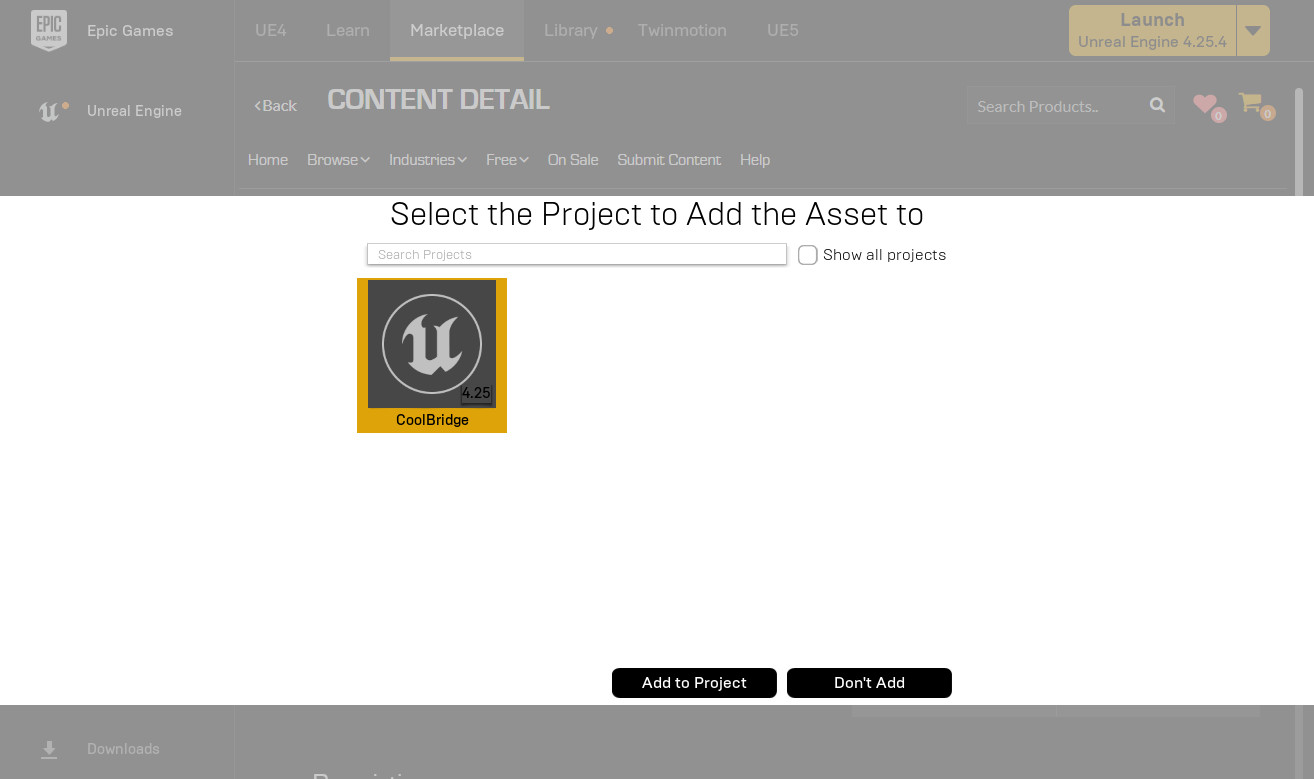
\includegraphics[height=225pt]{figures/egl_add_to_project_edit}
    \caption[Epic Games Launcher: Download assets to project]{
        In the Epic Games Launcher, this is the screen that allows you to download assets to a project.}%
    \label{fig:egl_add_to_project}
\end{figure}

As a final step, navigate to the Windows directory where the \ci{CoolBridge} project is located. By default, this should be in your \ci{Documents} folder under \ci{Unreal Projects}. If you look inside the \ci{Content} folder of the project, you'll notice that there is a folder named \ci{AutomotiveBridgeScene}. Note that this folder contains all of the assets that were just downloaded from the marketplace. Now go back to the \ci{CoolBridge} folder and delete the folders \ci{Intermediate}, \ci{Binaries}, \ci{Saved}, \ci{.vs}, and the file \ci{CoolBridge.sln}, if they are present.

That is all we needed to do using Windows. The remaining steps will all be done in Linux.

\subsection{Set the Project Up on Linux}
Copy the \ci{CoolBridge} folder to your Linux file system and place it in a directory of your choice. Create a folder in \ci{CoolBridge} named \ci{Plugins}, and place inside it a working copy of VTOL-AirSim (i.e., not broken) from one of your other Unreal Projects.

\section{Edit Project in Unreal Editor}\label{sec:edit_project_ueditor}
Launch Unreal Editor and open the \ci{CoolBridge.uproject} file. In the dialog, select \textbf{More Options} then \ci{Convert in-place}, and it will convert your project to work with your version of Unreal Engine on Linux. On the next dialog, click \textbf{Yes} to rebuild the modules.

When the project has been built and is opened in the editor, you should get a notification in the bottom-right that says \textit{Project file is out of date. Would you like to update it?} Select \textbf{Update}, and this will add an entry to the \ci{CoolBridge.uproject} file that contains the AirSim Plugin as part of the project. Also, before proceeding, go to \textbf{Edit > Editor Preferences}, and in the search box, type \texttt{CPU} and ensure that the setting \textbf{Use Less CPU when in Background} is unchecked.

In the \textbf{Content Browser}, navigate to the folder \ci{AutomotiveBridgeScene/Maps} and double-click on the level \ci{Bridge_P}. This will load the level in the editor. It may take a while to load the first time. When the Editor has loaded the level and finished compiling the necessary shaders, you should see a picturesque scene of a bridge in the \textbf{Level Viewport}.

\subsection{Configure the Project for VTOL-AirSim}
Let's make this level the default one in case we want to package it into a standalone application later. Go to \textbf{Edit > Project Settings}, then click \textbf{Maps \& Modes} in the left column. Change both the \textbf{Editor Startup Map} and the \textbf{Game Default Map} to be the current level, \ci{Bridge_P}. Close out of the project settings.

Next, in order to perform a VTOL-AirSim simulation when we use Play In Editor or when we launch the standalone application, we have to set the \textit{Game Mode} to be \ci{AirSimGameMode}. Do that by going to \textbf{Window > World Settings}, then in the \textbf{World Settings} panel in the lower-right corner, find the \textbf{GameMode Override} setting and change it to \ci{AirSimGameMode}.

\subsection{Place a Player Start Actor}

\begin{figure}[t]
    \centering
    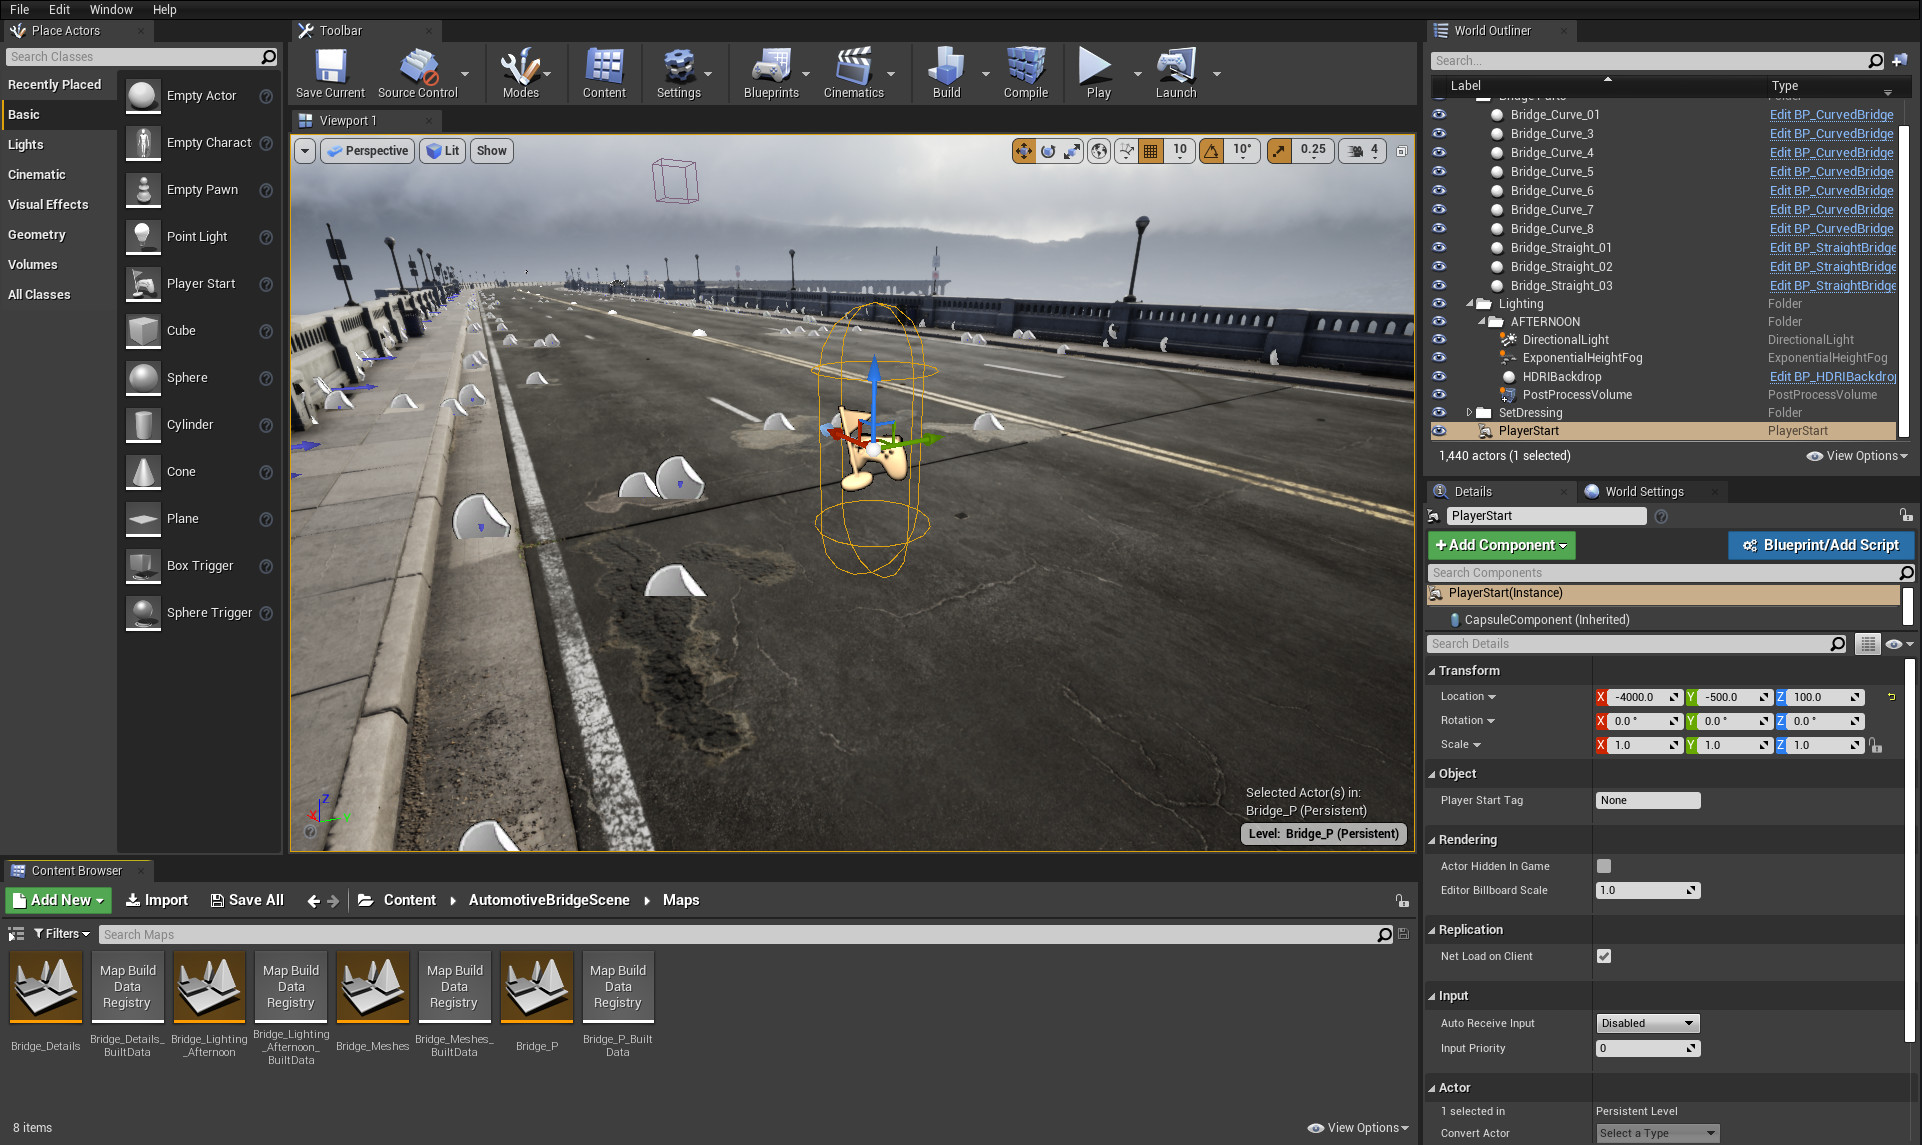
\includegraphics[width=\textwidth]{figures/ue4_bridge_playerstart}
    \caption[Custom environment in Unreal Editor]{
        The custom environment with a \textbf{Player Start} actor placed in the level.}%
    \label{fig:ue4_bridge_playerstart}
\end{figure}

Now we need to set where we want the vehicle to spawn in the world --- or, more precisely, where we want the global origin to be for VTOL-AirSim. \ci{AirSimGameMode} is configured to look for the \textbf{Player Start} Actor to set the global origin and spawn the vehicle; however, there is no \textbf{Player Start} Actor in this level, so we need to add one. In the \textbf{Place Actor} panel, find \textbf{Player Start} and drag it onto the \textbf{Level Viewport}. It should now appear in the \textbf{World Outliner} panel, and it should also have its attributes visible in the \textbf{Details} panel. While you may set the \textbf{Player Start} Location to wherever you like, we found a good starting position for this example to be the Location (X, Y, Z) values of (-4000.0, -500.0, 100.0). Set the \textbf{Player Start}'s Location attribute to be these values. You can double-click on the \ci{PlayerStart} Actor in the \textbf{World Outliner} to center the \textbf{Level Viewport} over its new location. After centering the view, the \textbf{Level Viewport} should look similar to Fig.~\ref{fig:ue4_bridge_playerstart}.

\section{Flight in New Environment}
We are ready to fly the tiltrotor aircraft in the level. First, make sure your settings file at the path \ci{~/Documents/settings.json} is set with \ci{"SimMode": "Vtol"}. Next, press \textbf{Play} in the editor, and in the \textbf{Level Viewport} you should see the tiltrotor aircraft spawn in the level. In a terminal, run the geometric controller example from Section~\ref{sec:vtol_geometric_control}. You should now see the tiltrotor flying through the custom environment, as shown in Fig.~\ref{fig:ue4_bridge_flying}.

\begin{figure}[h]
    \centering
    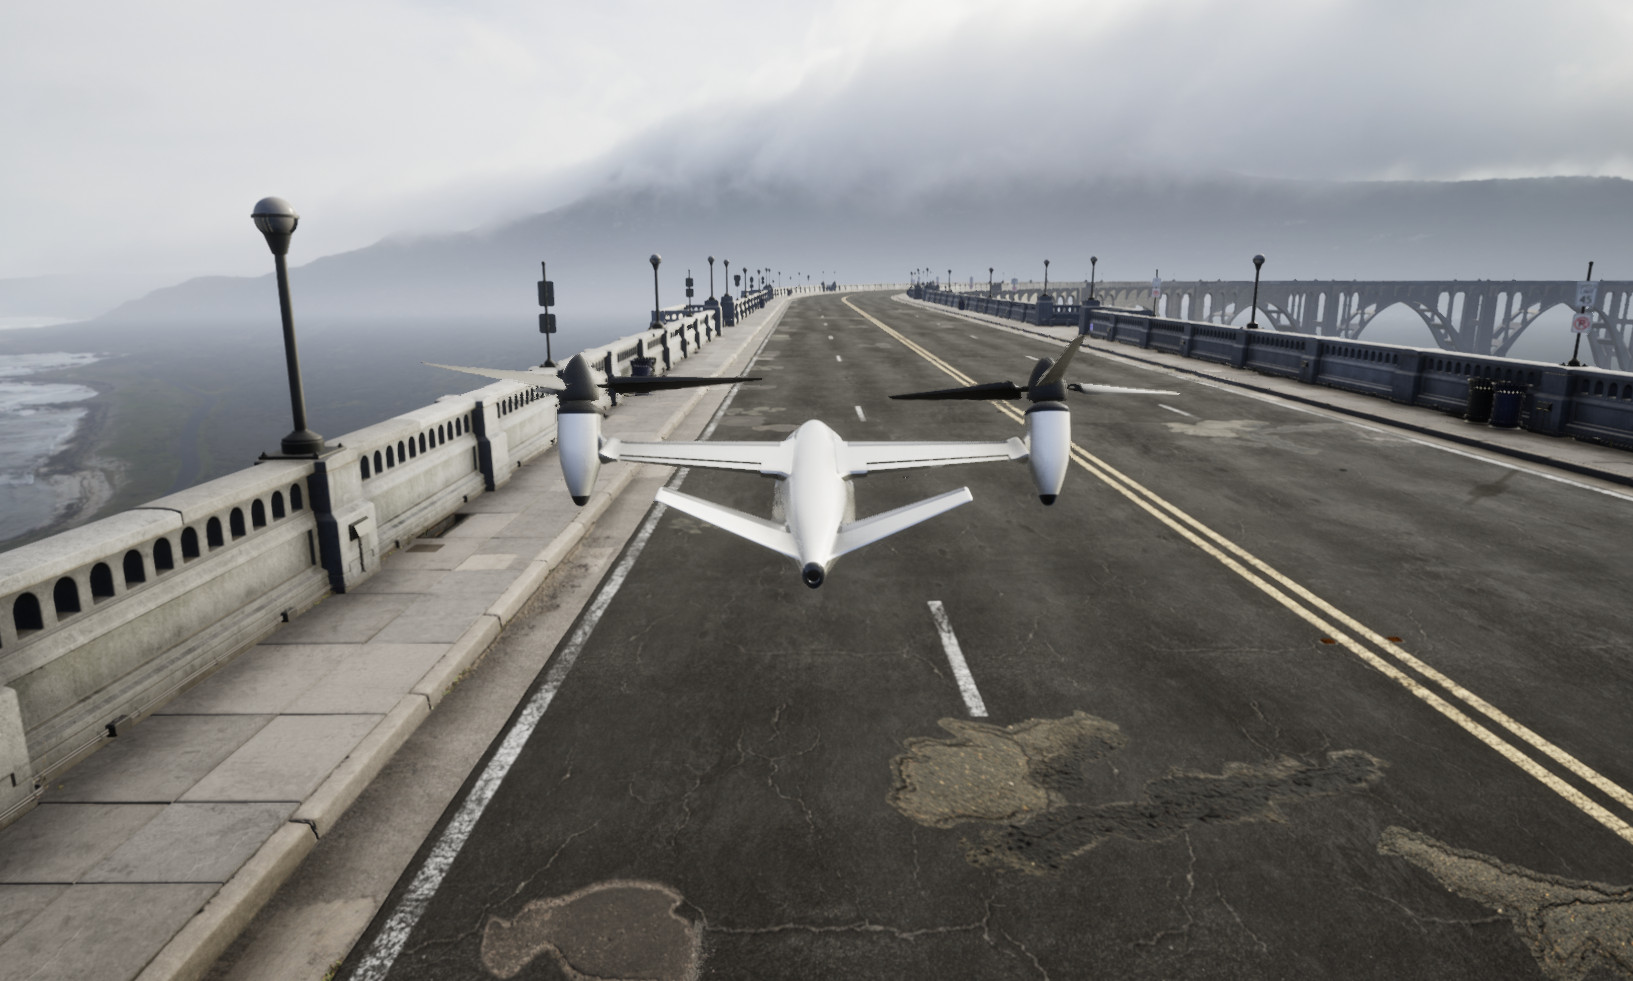
\includegraphics[width=\textwidth]{figures/ue4_bridge_flying}
    \caption[Tiltrotor flying in custom environment]{
        The tiltrotor aircraft flying in the \textit{Automotive Bridge Scene} custom environment.}%
    \label{fig:ue4_bridge_flying}
\end{figure}
%TC:envir minttcb [ignore] xall

\chapter{Conclusions and Future Work}\label{chp:conclusion}

Autonomous eVTOL aircraft have the potential to provide a new mode of air transportation for humans and cargo that is cheaper, more rapid and more efficient than has previously been possible. Simulation is key to the development of these aircraft, but there is currently a scarcity of simulation tools that have high-quality graphics, are publicly accessible, are easy to use, and which can simulate eVTOLs.

In this work, we contribute \textit{VTOL-AirSim}, a full integration of eVTOL aircraft into Microsoft AirSim. Our work includes new visual components that are packaged with VTOL-AirSim: a fully animated tiltrotor mesh, and a realistic city environment. We also contribute a tutorial on how to use VTOL-AirSim, and a guide on how to extend the capabilities of VTOL-AirSim. Finally, we demonstrate complete examples of creating custom aircraft and environments for VTOL-AirSim, so that others may customize it according to their needs.

This work aims to make VTOL-AirSim as accessible as possible to those seeking to use the simulator and to those who wish to increase its capabilities. It is our hope that others will find VTOL-AirSim to be a useful tool for simulating eVTOL aircraft in visually realistic environments. VTOL-AirSim has already been used in several research projects at the BYU MAGICC Lab. We hope that this trend will continue, and that future work will increase its reach even further.

\section{Review of Contributions}

A user guide for VTOL-AirSim can be found in Chapter~\ref{chp:userguide}. We give an overview of the additions made by VTOL-AirSim in Section~\ref{sec:vtolairsim} and its unique settings in Section~\ref{sec:settings_file}. In Section~\ref{sec:vtol_examples}, we give three complete examples of how to fly eVTOL aircraft: how to interface with a trajectory generator, geometric controller, and control allocation module in VTOLsim to send motor PWM commands (Section~\ref{sec:vtol_geometric_control}); how to set the vehicle's state via teleporting with an external dynamics simulation (Section~\ref{sec:vtol_teleport}); and how to interface with the PX4 Autopilot's VTOL controller to fly a mission (Section~\ref{sec:vtol_px4}).

In Chapter~\ref{chp:extending}, we show how to set up and use all the tools required for developing and extending VTOL-AirSim. Section~\ref{sec:unreal_setup} explains how to set up Unreal Engine on Linux, and Section~\ref{sec:vtolairsim_setup} explains how to set up VTOL-AirSim for development work. In Section~\ref{sec:vtolairsim_unreal}, we give a basic guide on working with VTOL-AirSim in the Unreal Editor.

We give complete examples of how to customize VTOL-AirSim with custom aircraft and custom environments in Chapters~\ref{chp:custom_aircraft} and~\ref{chp:custom_envs}, respectively. In Chapter~\ref{chp:custom_aircraft}, we show how to: obtain an aircraft mesh (Section~\ref{sec:meshes}), edit a mesh in Blender (Section~\ref{sec:blender_example}), import the mesh into Unreal Engine (Section~\ref{sec:import_mesh_ue4}), make a new Blueprint (Section~\ref{sec:blueprint}), and finally create a new \CC class for the custom aircraft (Section~\ref{sec:cpp_class}). Chapter~\ref{chp:custom_envs} details how to use the Epic Games Launcher on Windows to obtain assets from the Unreal Engine Marketplace (Section~\ref{sec:obtain_assets_windows}) and how to edit an Unreal Project with a custom environment in Linux using the Unreal Editor (Section~\ref{sec:edit_project_ueditor}).


\section{Future Work}
Our work of creating VTOL-AirSim is only the beginning of what can be done for the simulation of eVTOL aircraft in AirSim. There are a few ways in which VTOL-AirSim can be improved, and there are many things that can be added that would greatly increase its utility for several types of research projects. We present here a few examples of improvements that can be made.

First, the teleport functionality in VTOL-AirSim only works for setting the pose of the vehicle. Setting the tilt of the rotors with the teleport command, \ci{simSetVtolPose}, is broken. We attempted to implement this in code via a new function, named \ci{setPoseCustom}, to the \ci{TiltrotorPawnSimApi} \CC class. This function does successfully set the tiltrotor's pose in the data structure holding its physics state, but it appears that the current implementation for setting the rotor tilts is only successful for a brief moment until the motor outputs are overwritten in \ci{vtol_simple::Firmware::update()}, specifically by the call to \ci{board_->writeOutput()}. The firmware is updated at every iteration of AirSim's main loop, and since the firmware hasn't received any commands, it repeatedly sets the rotor tilts to zero, i.e., their nominal angle. Commands made by the AirSim client are executed on a separate thread from the main loop, and thus the two threads compete with one another to produce instantaneous, rapid shifting of the rotor tilts between their set values and their nominal angle. A solution could be to bypass the \ci{VtolSimple} firmware entirely, or to find a way to work with the firmware to set new motor outputs.

Second, while VTOL-AirSim includes support for tiltrotor aircraft, this is just one of several types of winged eVTOL. It also contains only one specific eVTOL model, the E-flite Convergence. Adding a new aircraft model is fairly straightforward, though it requires modifying the VTOL-AirSim source code and performing a source build. This is also how AirSim implements different multirotor models, so this is not unique to VTOL-AirSim; but it is more cumbersome than it needs to be. Ideally, the Convergence model would be the default, and a user could specify a parameter file that would be read at runtime to change which internal aircraft model is used. Adding support for other types of eVTOL would be a bit more difficult, but we designed VTOL-AirSim with adding other eVTOL types in mind, and there are empty functions left in the code that simply need to be implemented for another eVTOL type and it should work. The more time-intensive component would be to add a new aircraft mesh to represent the new eVTOL type, and if it is to be built in to VTOL-AirSim, how to specify which eVTOL type is desired in the settings file and then dynamically change the mesh of the vehicle.

Finally, it would be ideal for VTOL-AirSim to use a tiltrotor mesh which represents the actual dynamic model. This could be a different mesh which is a true tri-tiltrotor like the E-flite Convergence, or this could be a new dynamic model for a dual-tiltrotor, or a combination of both solutions.


%%%%%%%%%%%%% begin Bibliography %%%%%%%%%%%%%%%%%
\cleardoublepage{}
\bibliographystyle{IEEEtran}
\bibliography{refs} % Use your own BibTex file here

% Include appendix sections here: (or comment these lines out to have no appendices)
\appendix
%TC:envir minttcb [ignore] xall

\chapter{Miscellaneous Instructions}\label{apdx:misc_instructions}

% \section{Add a New Aircraft Configuration}\label{apdx:add_configuration}
% This section explains how one could change or add a new \textit{configuration} for the \verb|VTOL| vehicle type. A configuration is the

\section{Authentication for GitHub Using \texttt{gh} Client}\label{apdx:github_config}

An easy way to configure your Linux environment to clone, push, pull, etc.\ from GitHub repositories is to use the official GitHub CLI tool called \ci{gh}. First, go to \url{https://github.com/cli/cli/blob/trunk/docs/install_linux.md} and follow the instructions to install \ci{gh}. Then, in a terminal, run the command \ci{gh auth login}, which will guide you through a number of steps, for which you should do the following:

\begin{itemize}
    \item Choose \ci{GitHub.com}, then choose \ci{SSH}
    \begin{itemize}
        \item If you haven't generated a public SSH key previously, then choose ``yes'' at the prompt by pressing Enter, then press Enter again to leave passphrase blank
        \item If you already have a public SSH key, then choose it when prompted
    \end{itemize}
    \item Choose \ci{Login with a web browser}
    \item Copy the given code, then press Enter; this will open your web browser
    \item Authorize in web browser using the copied code
    \item Go back to the terminal, then press Enter to finish
\end{itemize}

You can now use either \ci{git} commands or \ci{gh} commands to interact with GitHub repositories. For example, to clone the AirSim repository, you can run either of the following:

\begin{minttcb}[title={Clone a GitHub Repository Option 1: \texttt{git}}]{bash}
    git clone git@github.com:microsoft/AirSim
\end{minttcb}
\begin{minttcb}[title={Clone a GitHub Repository Option 2: \texttt{gh}}]{bash}
    gh repo clone microsoft/AirSim
\end{minttcb}

For more information about connecting to GitHub with SSH, see the GitHub docs at \url{https://docs.github.com/en/authentication/connecting-to-github-with-ssh}.

\section{Advanced Setup for Python Virtual Environments}\label{apdx:adv_setup_python_venv}

You can place these bash functions in either your \ci{.bashrc} file or \ci{.zshrc} file, or in another file which is sourced by either of those files. Then, you can run, for example, the command \ci{workon airsim} to activate your Python virtual environment named \ci{airsim}. Run the command \ci{workoff} to deactivate your virtual environment.

\begin{minttcb}[]{bash}
    workon() {
        if [[ -n "$VIRTUAL_ENV" ]]; then
            deactivate
        fi
        source $HOME/.virtualenvs/$1/bin/activate
    }

    workoff() {
        if [[ -n "$VIRTUAL_ENV" ]]; then
            deactivate
        fi
    }
\end{minttcb}


\section{Alternate Method for Moving Mesh Origins in Blender}\label{apdx:blender_origins_alt}
In the past, we have accomplished getting the correct pivot points in Unreal Engine using a different method than the procedure outlined in Section~\ref{sec:blender_example}. The method is to:

\begin{itemize}
    \item create separate \ci{.blend} Blender files for each object mesh that you want to animate on the aircraft (e.g., engines, propellers, ailerons)
    \item Do the following for each Blender file:
    \begin{itemize}
        \item If there are multiple meshes, choose one as the root object and make the other objects the children of it using the drag, then \texttt{Shift+Alt}, then drop technique
        \item Hold pointer over the Viewport and press \texttt{A} to select all objects
        \item Select \textbf{Object > Set Origin > Origin to Geometry} to set origins of the meshes to their geometric centers
        \item Select \textbf{Object > Snap > Cursor to World Origin}
        \item Select the object, or, if there are multiple objects, select the root object
        \item Select \textbf{Object > Snap > Selection to Cursor}
        \item If there are any nonzero values for the Location of the object (or root object), apply the Location by holding the pointer over the Viewport and pressing \texttt{Ctrl+A} then clicking \textbf{Location}
        \item Repeat the process to apply all Rotations
        \item Export to FBX file with default settings under the \textbf{Transform} section:
        \begin{itemize}
            \item \textbf{Up} set to \textbf{Y Up}
            \item \textbf{Use Space Transform} checked
            \item \textbf{Apply Transform} unchecked
        \end{itemize}
    \end{itemize}
    \item After finishing the exports, import each FBX file into UE4
    \item Create a Blueprint with the aircraft's body as the Root Component
    \item Add the other meshes to the Blueprint
    \item Manually set each component's Location to where they should be relative to the aircraft body
\end{itemize}

%TC:envir minttcb [ignore] xall

\chapter{Further Information}\label{apdx:further_info}

\section{List of Available Prebuilt Environments for Linux}\label{apdx:list_of_envs}

This list is based on the available environments as of AirSim v1.5.0.

\begin{itemize}
    \item AbandonedPark --- contains a few scattered objects such as a ferris wheel and some swings
    \item Africa --- open ground covered in patches of water, bordered by trees
    \item AirSimNH --- a suburb with diverse features such as houses, cars, trees, and mobile animals
    \item Blocks --- very simple example world with large geometric shapes scattered around
    \item Building99 --- inside of a mall with a number of people walking about
    \item LandscapeMountains --- large, open, and detailed mountain environment
    \item MSBuild2018 --- tennis courts, trees, and buildings making up the Microsoft campus
    \item TrapCamera --- an open and configurable world with some animated, stationary animals
    \item ZhangJiajie --- an area above the clouds with large, stone pillars of varying heights scattered about
\end{itemize}


\section{Blender for Work Involving Meshes}\label{apdx:blender}

Blender is an extremely powerful 3D modeling application that is open-source, completely free, and has full Linux support~\cite{Blender2021}. For these reasons, we highly recommend using Blender for any work that involves editing, producing, or preparing meshes for Unreal Engine. The examples in this text using Blender were done with Blender v2.93.5. Our experience has been good with regards to modifying a mesh and exporting it from Blender in FBX format for import into UE4. While not perfect, it is the only solution we know of that works reliably. This is the pipeline we used for the tiltrotor mesh that comes with VTOL-AirSim. We also used Blender to make a number of modifications to the mesh.

On Ubuntu 20.04, there are three ways to install Blender:

\begin{enumerate}
    \item via their website at \url{https://blender.org/download} (Recommended)
    \item via \ci{apt} with the command \ci{sudo apt install blender}
    \item as a Snap application with the command \ci{sudo snap install --classic blender}
\end{enumerate}

We recommend the first option because it will get you the latest version of Blender (as will the third option, if you use Snap applications). The examples in this text were tested using the latest version of Blender, v2.93.5 --- however, at the time of this writing, the latest version of Blender available via \ci{apt} is v2.82. If you do use Blender v2.82, we cannot guarantee that the examples will work according to the instructions we provided.

If you install via the official \url{blender.org} website, extract the archive file to somewhere on your machine and launch blender by running the \ci{blender} executable found inside the extracted directory.

\section{Unreal Engine Paths And References}\label{apdx:unreal_paths}
The way that Unreal Engine references paths in a project is rather unconventional. It is important to understand how it works if you are going to do work in the Unreal Editor. The following list explains the different path names that UE4 uses and what you can substitute them with to get the corresponding path on your file system. In the examples given, we will assume a project named \ci{Blocks}; the absolute path to the project is omitted for brevity.

\begin{itemize}
    \item Prefix \ci{/Game/}: substitute with \ci{<project>/Content}
    \begin{itemize}
        \item Example path: \ci{/Game/Flying/Meshes}
        \item refers to: \ci{Blocks/Content/Flying/Meshes}
    \end{itemize}
    \item Prefix \ci{/AirSim/}: substitute with \ci{<project>/Plugins/<plugin_dir>/Content}
    \begin{itemize}
        \item Note: inside UE4, the name of the VTOL-AirSim Plugin is \textbf{\texttt{AirSim}}. UE4 does not read the directory name; it reads what is inside the \ci{AirSim.uplugin} file, which we have kept as \texttt{AirSim} for compatibility with the base AirSim repository. Thus, \ci{<plugin_dir>} could be \ci{Plugins/AirSim} or \ci{Plugins/vtol-AirSim}.
        \item Example path: \ci{/AirSim/VTOL/Tiltrotor/Meshes}
        \item refers to: \ci{Blocks/Plugins/vtol-AirSim/Content/VTOL/Tiltrotor/Meshes}
        \item Example path: \ci{/AirSim/Blueprints}
        \item refers to: \ci{Blocks/Plugins/AirSim/Content/Blueprints} (if using the default AirSim plugin rather than VTOL-AirSim)
    \end{itemize}
\end{itemize}

In the \textbf{Content Browser}:

\begin{itemize}
    \item \ci{Content}: substitute with \ci{<project>/Content}
    \begin{itemize}
        \item Same as \ci{/Game/} above
    \end{itemize}
    \item \ci{AirSim Content}: substitute with \ci{<project>/Plugins/<plugin_dir>/Content}
    \begin{itemize}
        \item Same as \ci{/AirSim/} above
    \end{itemize}
\end{itemize}


\end{document}